\chapter{Implementation}
\label{cha:implementation}
% short overview; why web -- use references!
% speak about quick prototyping possibilities and how it's easier to roll out updates and how nobody needs to download an app on their phone to interact with the presentation
% say something about open source and why all the code is online on github!
%
%
%
% In Implementation: Give overview of how it works: server on presenter computer (like in Office Social!), IP address is distributed to viewers, they go there and can then follow the presentation.

% Every slide deck is generally created with HTML and JavaScript and styled with CSS, individual slides are composed of JSX-components (see chapter \ref{cha:implementation}). This means the speaker has to have some knowledge of front-end web technologies to be able to author slides.
% The finished slide deck is then either uploaded to a publicly accessible web server or, if all audience members are connected to the same wifi, can be served locally from the speaker's computer.

This chapter dives into the technical implementation details of the thesis project and gives an overview of the used technologies and explains why these were chosen over others. Like many other projects in this area \cite{Bry:Backstage, Cheng:TreebasedOnlinePresentations, Esponda:ElectronicVotingOnTheFly, Inoue:RealTimeQuestionnaire, Teevan:MobileFeedbackDuringPresentation, Triglianos:InteractiveWebPresentationsImpress}, the project is realised as a web application. This has many advantages, from modern web technologies' quick prototyping capabilities to the web's general cross-platform and cross-device nature, the project has benefitted from the dynamicity of the internet and the rapid evolvement of JavaScript over the past years.
Although native sharing features of smartphones cannot be used due to the choice of platform, the advantages that come with this decision outweigh the disadvantages, as I like to think, for both users and developers: as nobody has to download any apps to their devices, it is easier to bring the audience to use the developed application \cite{Triglianos:InteractiveWebPresentationsImpress}. The major advantages for developers on one hand is the ability to only concentrate on one platform instead of developing different applications for different operating systems, on the other hand the web is built for rapid prototyping as it is extremely easy and fast to roll out new updates, without distributing them through the App Store or Play Store and without the need for users to manually update them. The chosen JavaScript library React, however, offers the possibility to cross-compile applications to different devices using React Native, which should make it fairly easy to port the existing web application in the future.

As it was important to achieve fast response times and because \emph{WebSockets} have successfully been deployed in the real-time features of other presentation tools \cite{Inoue:RealTimeQuestionnaire, Triglianos:InteractiveWebPresentationsImpress}, this technology has also been used in this thesis project, to handle the communication between clients and server.

A few words should also be said about the distribution of this project. Without the vibrant open-source community, many of the frameworks and libraries used in this project would not exist. For this reason and to give back to this community, all the libraries developed during this project are published as open-source on my GitHub profile\footnote{\href{https://github.com/irisSchaffer?tab=repositories}{\textsf{https://github.com/irisSchaffer/}}} and freely available for anyone to use.

\section{Project Scope}
\label{sec:implementation-scope}
% What's the general scope of the project? Why is everything on the client and 
% not the server? etc.
Before jumping into technical details, the scope of the project should be discussed. As the aim of the present work is to explore ways of incorporating mobile devices into presentation workflows, the goal of the project was to use an easily extensible presentation library to then build the mechanisms discussed in the previous chapter on top of it.
As the focus was placed on the interaction possibilities between speaker and audience, the creation of the presentation for the speaker or the management of slides and presentations were out of scope. Therefore the server used for connecting different users to the presentation was kept as simple as possible, allowing any potential other developer to work with their own servers and technology stacks.

In total, a system with several ways of interacting with the presentation from mobile or desktop devices was created, putting emphasise on mobile-optimised views and navigation possibilities. This system includes synchronisation of navigation state and state changes between viewers and speaker, the possibility to add sub-slides during the presentation for the audience, a speaker-view showing the next slides and controls, real-time voting (both created on-the-fly and prepared beforehands) and the possibility to create different paths through the presentation. In the following the technologies used in the project will be analysed and described to then discuss implementation details, problems and solutions of the mentioned components.

\section{Technologies}
\label{sec:implementation-technologies}
% Which technologies were chosen and why?
% How do they generally work? To a level on which the reader can
% understand the rest of the implementation details
% A few words about responsive design and media queries would probs be good
% a few words about babel and es6

The project generally tries to follow best-practices in web development and utilises modern CSS3 and JavaScript features and frameworks. The software is written in ECMA\-Script\-2015, makes use of the \emph{node package manager}\footnote{\url{https://www.npmjs.com/}}(short \emph{npm}) for managing dependencies and \emph{Babel} to transpile to ECMA\-Script\-5. Additonally to relying on CSS3 features, this project also uses \emph{Sass}\footnote{\url{http://sass-lang.com/}} as a CSS pre-processor. Media-queries allow for mobile-friendly views.

On the front end, which this project focuses on, the JavaScript library \emph{React} is the framework of choice, additionally applying the \emph{reactive programming} paradigm using \emph{RxJS} to allow for a simpler interface for event-driven operations. The communication between client and server is handled by \emph{socket.io}\footnote{\url{http://socket.io/}}.
This section tries to introduce the reader to the main technologies used to establish a base on which the following technical implementation details can be understood.

\subsection[ECMAScript2015 and Babel]%
             {ECMAScript2015 and Babel%
             \protect\footnote{\url{https://babeljs.io/}}}%
\label{sec:implementation-technologies-es6}
% it's a recommendation, but it takes long until browsers implement it and users update their browsers.
JavaScript undoubtly is an integral part of front end web development and since the emergence of server-side JavaScript with Node.js\footnote{\url{https://nodejs.org/en/}} and its package manager npm has developed into a programming language widely used by web developers \cite{gpm-meta-transcompiler}. Both PYPL\footnote{\url{http://pypl.github.io/PYPL.html}} and TIOBE\footnote{\url{http://www.tiobe.com/tiobe_index}} programming language indices rank JavaScript among the top 10 programming languages (PYPL at 5, TIOBE at 7 at the time of writing) \cite{gpm-meta-transcompiler}. Stack Overflow's 2015 Developer Survey even places JavaScript as the number 1, most-used programming language with 54.4\% and JavaScript, Node.js and AngularJS\footnote{\url{https://angularjs.org/}} all three rank amongst the top 5 languages developers expressed an interest in developing with \cite{stackoverflow-developer-survey}.

However, like any front end technology, JavaScript suffers from slow end user adoption, as a multitude of browser versions exist for different devices and operating systems and many people still do not auto-update their browsers. Another factor is the time it takes for browser-vendors to implement new ECMAScript standards (the standard behind JavaScript) and roll out said updates. This is exactly what is happening with the new ECMAScript standard, ECMA-262, commonly known as ECMAScript 2015 or ES6: Although the General Assembly has adopted the new standard in June 2015 \cite{ecma2015}, \emph{Kangax' ECMAScript compatibility tables}\footnote{\url{https://kangax.github.io/compat-table/es6/}} still show a fairly low level of support, especially among mobile browsers. ES6 makes JavaScript easier and more efficient to write by providing new semantics for default values, arrow-functions, template-literals, the spread operator or object destructuring \cite{es6}. It also makes JavaScript easier to understand and safer to develop with the introduction of block-scoped variables (\texttt{let} and \texttt{const}) and finally offers native support of modules and promises \cite{es6}.
As these features are all included in the new ECMAScript standard, it is safe to assume browser-vendors will implement them in the near future. Until then, developers who want to already make use of them, can \emph{transpile} ECMAScript 2015 code to ECMAScript 5, which is exactly what Babel does. With almost $750.000$ downloads in April 2016 \cite{npm-babel} and companies like Facebook, Netflix, Mozilla, Yahoo or PayPal using this transpiler \cite{babel-users}, Babel is the de facto standard solution to transpile to ECMAScript 5 and was also chosen for this project.

\subsection{Reactive Programming}
\label{sec:implementation-technologies-rxjs}

Another problem with JavaScript, although integral part of the reason for its high popularity, is its asynchronous nature. Especially when working with highly interactive parts, the prime example being user interfaces, sequential programming quickly gets too inflexible to handle complex, event-driven applications \cite{reactive-programming-survey}. The same is true for the server where the possibility to concurrently serve a multitude of different clients is crucial. In these cases JavaScript offers \emph{event listeners} -- functions called once a certain event happens. However, these event listeners or \emph{asynchronous callback} \cite{reactive-programming-survey}, oftentimes execute more asynchronous code and in turn have to wait for another event, and another one, and another one..., which can result in something known and dreaded by most any JavaScript developer: \emph{Callback Hell} (see programm \ref{prog:implementation-technologies-rxjs-callback-hell}).

\begin{program}
\caption{\emph{Callback Hell} -- Nested callbacks in JavaScript. Simplified method taken from a previous project, which authenticates a user, creates a new google calendar for them and then saves the user to one's own database, to then redirect them. \texttt{\{...\}} is used to shorten the code, error-handling was also omitted in the example for simplicity.}
\label{prog:implementation-technologies-rxjs-callback-hell}
\begin{JsCode}
router.get('/callback', function(req, res, next) {
  var code = req.query.code;
  var name = JSON.parse(req.query.state);

  // get token from oauth library
  oauth2Client.getToken(code, function (err, tokens) {
    // load configuration
    Configuration.findOne({}, function (err, configuration) {
      var calendar = google.calendar('v3');
      // save to google calendar
      calendar.calendars.insert({...}, function (err, cal) {
        var member = new Member({...});
        // save member to own database
        member.save(function(err, member) {
          return res.redirect(getRedirectionUrl(name) + '&success=true')
        });
      });
    });
  });
});
\end{JsCode}
\end{program}

Different approaches have been employed to lower the hurdle of writing asynchronous code, one of them being \emph{promises}: A promise is a value, yet to be computed \cite{reactive-vs-promises}. A promise can be a) pending (if it has not been assigned a value yet), b) resolved (if it has been assigned a value) or c) rejected (if an error occurred). With ECMAScript 2015 promises, these objects can then be queued using the \texttt{then} keyword, to execute asynchronous code in a certain sequence (see programm \ref{prog:implementation-technologies-rxjs-promises}).

\begin{program}
\caption{\emph{Promises} -- Simple example of chaining ECMAScript 2015 promises with \texttt{then} and \texttt{catch}.}
\label{prog:implementation-technologies-rxjs-promises}
\begin{JsCode}
var promise = new Promise(function(resolve, reject) {
  asyncCall(function(error, data) {
    if (error) {
      reject(error); // reject the pending promise
    } else {
      resolve(data); // resolve the pending promise
    }
  })
})

promise
  .then(function(data) {
    // this is executed after asyncCall returns
    // other asyncronous calls can be placed here
  })
  .catch(function(error) {
    // this is executed if an error occurs somwehere along the way
  })
\end{JsCode}
\end{program}

However, promises can still create nested callbacks, especially when chaining promises that rely on other promises' resolution \cite{reactive-vs-promises}. This is where \emph{reactive programming} comes in: The reactive programming paradigm works with streams of events, in which every event is handled as a new value and all other parts depending on this value are re-computed upon arrival of such a new value. To demonstrate this I would like to use Bainomugisha et al.'s illustrative example of a simple addition \cite{reactive-programming-survey}:

\begin{JsCode}
let v1 = 1;
let v2 = 2;
let v3 = v1 + v2;
\end{JsCode}
%
In sequentially executed code, \texttt{v3} will hold the value $3$, no matter if or how \texttt{v1} or \texttt{v2} change. In reactive programming, however, \texttt{v3} will be re-computed as soon as either one of the values it depends on changes \cite{reactive-programming-survey}. This way for a drag-and-drop feature, for example, the move of the mouse, continuously sending its location, could directly alter the position of an element in a page. JavaScript does not directly support reactive programming, but other, more functional languages, which can be transpiled to JavaScript, do. Another way of adding reactive programming concepts to JavaScript is using a library, such as \emph{Bacon.js}\footnote{\url{https://baconjs.github.io/}} or the one chosen for this project, \emph{ReactiveX}\footnote{\url{http://reactivex.io/}}. ReactiveX provides libraries for a multitude of different programming languages, C#, C++, Java and of course JavaScript among them. The latter, called \emph{The Reactive Extensions for JavaScript} or short \emph{RxJs}, allows for the simple creation of event streams (\emph{Observables}) from browser events or promises directly and uses the same method names JavaScript developers are familiar with from array-methods, most notably and well-known \texttt{map}, to apply a method to every element in the incoming stream and \texttt{filter}, to only let a subset of events pass. These methods can be chained to sequentially alter a value (see programm \ref{prog:implementation-technologies-rxjs}).

\begin{program}
\caption{\emph{RxJS} -- simplified example of the touch controls used to swipe to the next or previous slide. An Observable is created from the browser's \texttt{touchmove} event and is then transformed with \texttt{map} and \texttt{filter}, to in the end call the \texttt{navigate()} method with the direction the user swiped into.}
\label{prog:implementation-technologies-rxjs}
\begin{JsCode}
this.moveObservable = Observable.fromEvent(document, 'touchmove')
  // data: event object with array of touches
  .filter(this.touchStarted) // only procede if touchstart is set to true
  .map(this.toXY) // transform initial event data to latest touch's xy position
  // data: \{x: xPosition, y: yPosition\}
  .map(this.toDirection) // transform xy position to direction literal
  // data: right/left/up/down
  .do(this.resetTouchStart) // set this.touchStarted to false
  // data: right/left/up/down
  .subscribe(this.navigate) // call this.navigate() with direction data
\end{JsCode}
\end{program}

Additionally to Observables, RxJs also knows \emph{Subjects}, which combine both a source of events and a consumer of such. Subjects are Observables, but also Observers at the same time and can be used to broadcast values to several consumers \cite{rxjs-docu}.

\subsection[React]%
             {React%
             \protect\footnote{\url{https://facebook.github.io/react/index.html}}}%
\label{sec:implementation-technologies-react}
% explain base concept of having re-usable components and how they are defined!
% get some HTML code in there :)

As this project concentrates on the front end, a mature JavaScript framework was searched for. After previous experience with the big and complex but slow AngularJS, and because of promising performance benchmarks \cite{react-benchmarks} and simply to explore new JavaScript libraries, I decided to give React a try. Since Facebook started developing React in 2013, it has challenged existing approaches and set new standards in front end web development \cite{introduction-to-react}. Instead of creating an entire MVC framework for the front end, React really concentrates on the view by offering a way of creating independent, lightweight view components. This gives React the huge advantage of beating other front end frameworks by far in performance benchmarks \cite{react-benchmarks}. Moreover, \emph{React Native}\footnote{\url{https://facebook.github.io/react-native/}} would make it possible to port the application to different mobile operation systems fairly easily.

The arguably most important method these re-usable, lightweight components implement is the \texttt{render} method, defining what HTML or JSX\footnote{\url{https://facebook.github.io/jsx/}} should be rendered by the browser:
\begin{JsCode}
export default class HelloWorld extends Component {
  render() {
    return (<h1>Hello World!</h1>)
  }
}
\end{JsCode}
%
The created Component can then be rendered into the virtual React DOM, JSX makes it possible to simply use the name of the component to create it:
%
\begin{JsCode}
ReactDOM.render(
  <HelloWorld />,
  document.getElementsByTagName('body')[0]
)
\end{JsCode}
%
This would simply put an \texttt{h1} element with the text \texttt{Hello World!} into the \texttt{body} element of the HTML page. Additionally to the \texttt{render} method, components also have a \emph{state} and \emph{properties} (\texttt{props}), through which they can communicate with other components and maintain their internal state. \texttt{props} are passed in to the component during creation, in JSX this can be achieved by simply passing them in as XML attributes:
%
\begin{JsCode}
  <HelloWorld greeting="Hi" />
\end{JsCode}
%
This could in turn be used in the \texttt{HelloWorld} component's \texttt{render} method:
%
\begin{JsCode}
  render() {
    return (<h1>{this.props.greeting} World!</h1>);
  }
\end{JsCode}
%
The children of a component are also available through \texttt{this.props.children}. The \texttt{state} variable, on the other hand, is responsible for handling internal updates e.g. through user interaction \cite{react-docu}. To alter the state, the method \texttt{setState} can be used, which will cause an update and re-rendering of the component. So if in the above example, the word ``World'' should be changed to something else by the user, a text field with an event handler can be added inside the component (see program \ref{prog:implementation-technologies-react-state}).
%
\begin{program}
\caption{Example code snippet using state in a React component. Whenever the text input changes (i.e. a user types something), the \texttt{update()} method will be called and set the state and cause a re-render.}
\label{prog:implementation-technologies-react-state}
\begin{JsCode}
// set default state and props...

componentWillMount() {
  // create observable from change event on input
  this.observable = Observable.fromEvent('change', this.refs.input)
    .pluck('target', 'value') // extract input text
    .subscribe(this.update) // call update with value
}

componentWillUnmount() { this.observable.unsubscribe() }

update(text) { this.setState({name: text}) }

render = () => (
  <div>
    <h1>{this.props.greeting} {this.state.name}!</h1>
    <input value={this.state.name} ref="input" />
  </div>
)
\end{JsCode}
\end{program}
%
Now, whenever a user changes the text in the \texttt{input} field, the RxJS Observable will receive a new value (a change event). The \texttt{value} of the field is extracted on line $6$ of program \ref{prog:implementation-technologies-react-state} and used to then update the state in the \texttt{update} method, which is implicitly called with the value passed through the Observable chain.

The two methods \texttt{com\-po\-nent\-Will\-Mount}, \texttt{com\-po\-nent\-Will\-Un\-mount} as well as \texttt{com\-po\-nent\-Did\-Mount}, \texttt{should\-Com\-po\-nent\-Up\-date}, \texttt{com\-po\-nent\-Will\-Up\-date}, \texttt{com\-po\-nent\-Did\-Up\-date} and \texttt{com\-po\-nent\-Will\-Re\-ceive\-Props} are \emph{lifecycle methods}, called whenever the component is created, updated or destroyed.

As an end note on React, and a transition to the core presentation library, I want to add that React components can be nested, which is at the core of the project developed for the present thesis. To make it as easy as possible for other developers to use the created libraries, a presentation is built just as a usual HTML page, using JSX to reference the custom React components, as will be shown later this chapter in program \ref{prog:implementation-client-presentation}.

\subsection[unveil.js]%
             {unveil.js%
             \protect\footnote{\url{https://github.com/ostera/unveil.js}}}    
\label{sec:implementation-technologies-unveil}
% explain how this was developed together with Leandro, explain general parts like router, navigator, UnveilApp
% Give overview over controls in here.
% Also talk about the mobile style sheets / responsive design and the TouchControls, which I also implemented alone.
% (mention that this part is unit tested with jest(https://facebook.github.io/jest/))

As a presentation layer, this project uses the open-source JavaScript library \textit{unveil.js}, which was developed by Leandro Ostera and myself in the beginning of the project and which I extended and adapted to my needs in an own fork\footnote{\url{https://github.com/irisSchaffer/unveil.js}} during the project. This fork will be covered in section \ref{sec:implementation-unveil} of this chapter, until then, a short overview of the different parts of unveil.js is given and key concepts of the library are discussed. Screenshots of what unveil.js looks like can be found in figure \ref{fig:implementation-technologies-unveil-screenshots}.
%
\begin{figure}
\centering
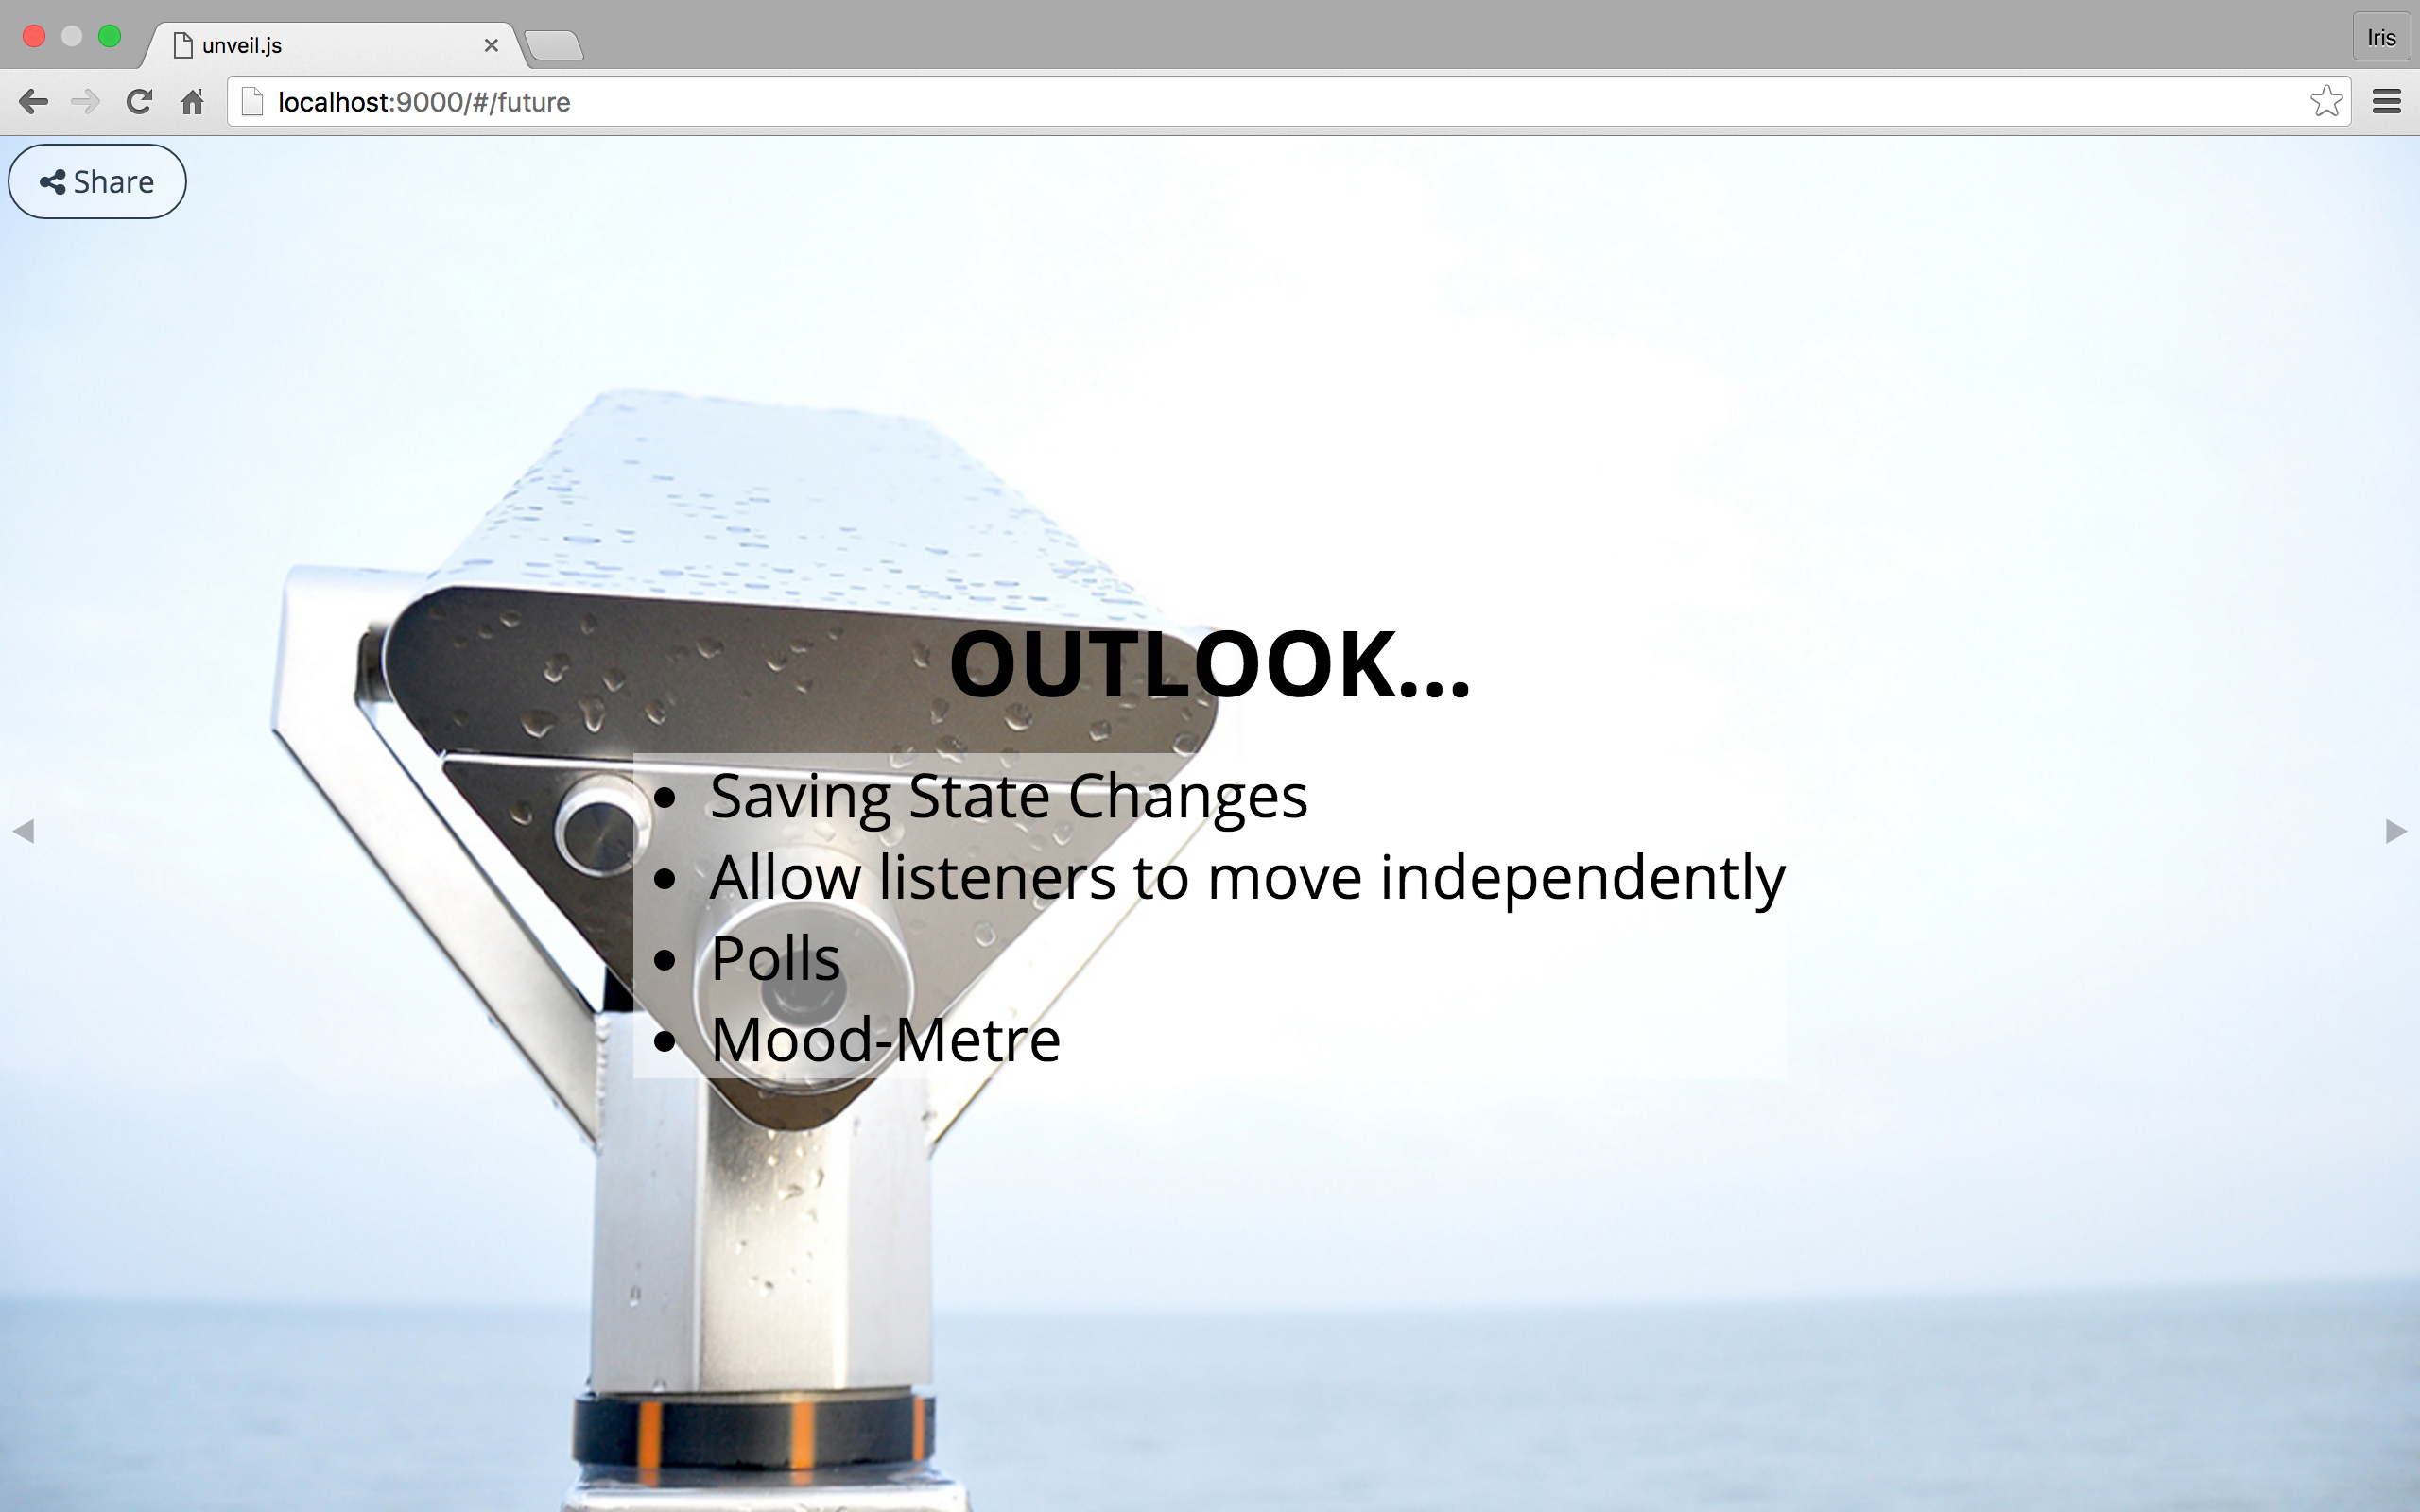
\includegraphics[width=0.65\textwidth]{presentation-screenshot}
\caption{Screenshot of an example slide with unveil.js, using interactive extensions discussed in section \ref{sec:implementation-interactive}.}
\label{fig:implementation-technologies-unveil-screenshots}
\end{figure}
%
Generally, unveil.js operates on a $2$-dimensional slide-space: Every slide can have a next and previous slide in $x$, as well as in $y$-direction. To generate the $y$ axis, slides can be nested in other slides. These slides have an optional unique name as well as an index in the slide-tree, which they are identified by. As shown in program \ref{prog:implementation-client-presentation}, slides are created inside the component \texttt{UnveilApp}, the core of unveil.js. This component configures and sets up the entire application based on optional configuration passed in as properties.
There are a few concepts unveil.js is built around to allow for extensibility and configurability, namely \emph{presenters}, \emph{controls} and \emph{modes}:
%
\begin{itemize}
\item \textbf{Presenters} define the way slides are rendered, e.g. show notes, upcoming slides or hide them.
\item \textbf{Controls} control a part of the application, e.g. navigating from one slide to the next using the arrow keys on the keyboard.
\item \textbf{Modes} are what allows a speaker to have a different presenter and controls from an audience member. Each mode defines its own presenter and set of controls, the mode is determined by the url query parameter \texttt{mode}.
\end{itemize}
This allows anybody using unveil.js to define new modes, presenters and controls and thereby extend the base library as they wish. A few of these are already defined, namely a default \texttt{Presenter}, \texttt{UIControls} to navigate using buttons, \texttt{KeyControls} to navigate using the keyboard and \texttt{TouchControls} to navigate with swipe-gestures on touch screens. In section \ref{sec:implementation-client}, modes for the audience (\emph{default}), the speaker (\emph{speaker}) and for use on the projection device (\emph{projector}) will be introduced.

For these controls and the entire presentation to be navigatable, \texttt{Un\-veil\-App} is responsible for the creation of two very important classes: \texttt{Router} and \texttt{Navigator}. These can be defined outside and passed into \texttt{UnveilApp} as properties, allowing users to customise their navigation logic.
%
The \texttt{Router} is the class handling everything connected to the current url. It receives the slide-tree and can compute the indices of a slide by its name and vice versa. Whenever the browser history changes, the router finds the corresponding slide-indices, computes an array of possible directions to go into from this slide and propagates the event to \texttt{UnveilApp}, which can then re-render the application.
\texttt{Navigator}, in turn, receives these directions and is responsible for the mapping of directions (\emph{left}, \emph{right}, \emph{up}, \emph{down}) to slide-indices. Controls know the navigator and can push new directions to the navigator subject, thus starting the navigation process described in detail in figure \ref{fig:implementation-technologies-unveil-navigation}.

\begin{figure}
\centering
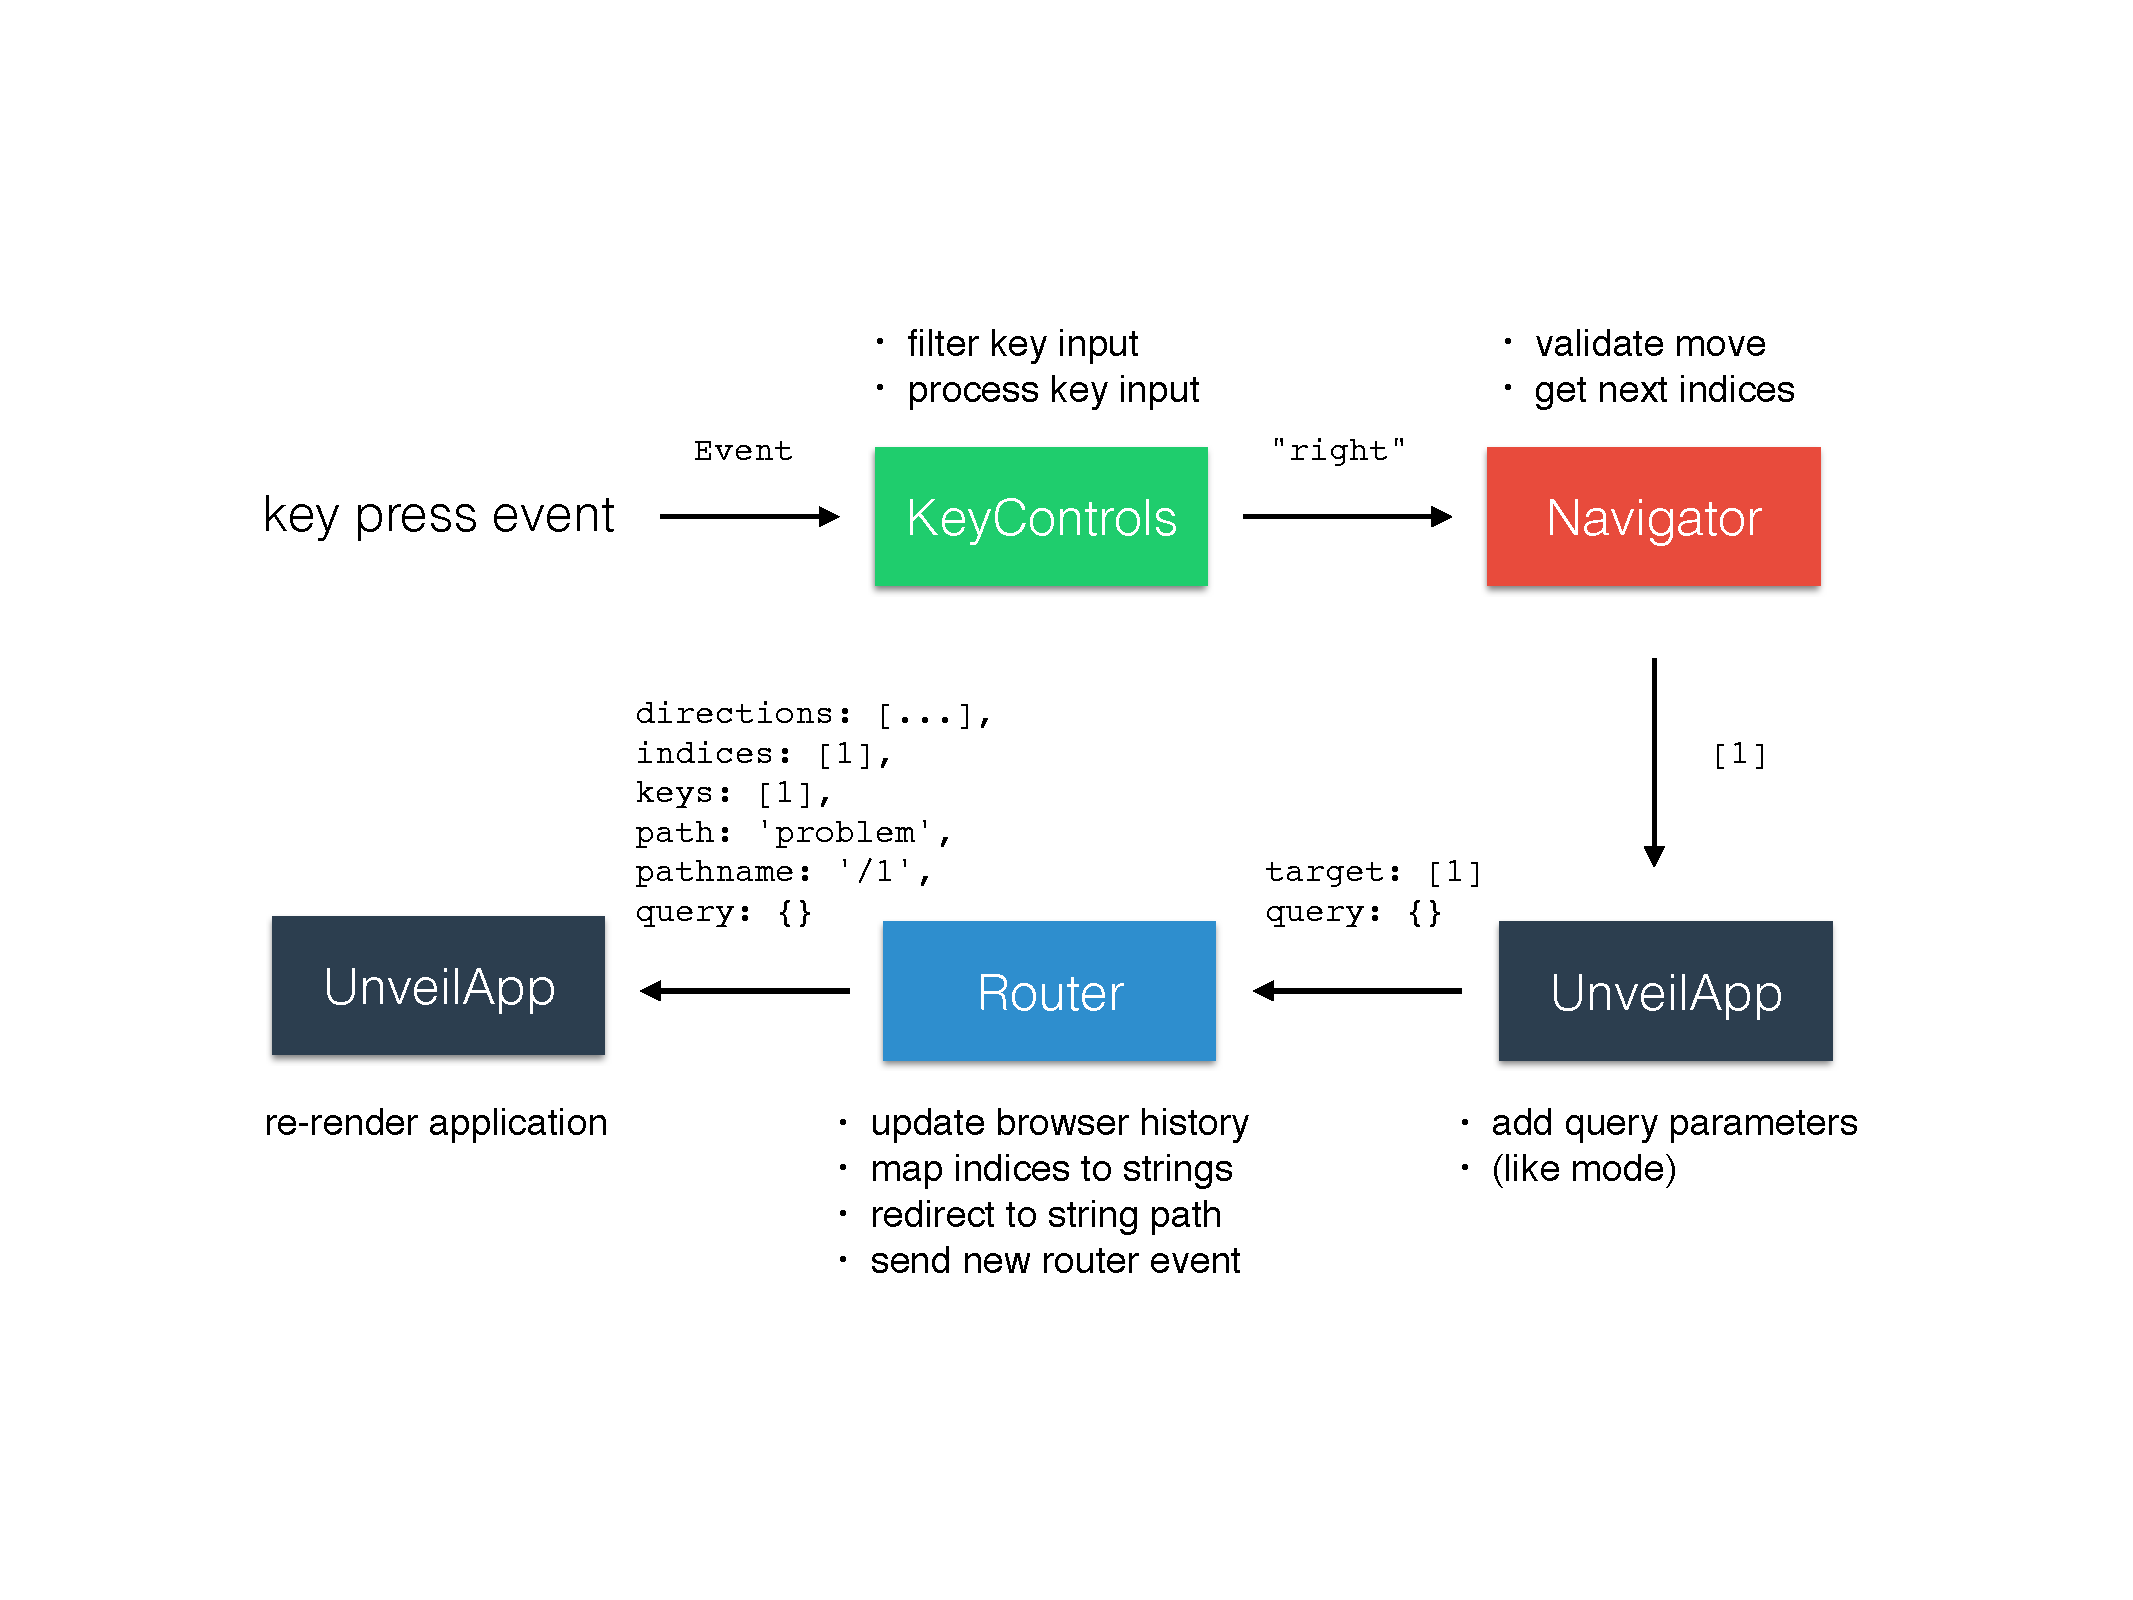
\includegraphics[width=.85\textwidth]{navigation}
\caption{Navigation pipeline from user's key press to re-render of the presentation. The monospaced text next to the arrows symbolises the data transmitted. \texttt{KeyControls} listen for key events and process them, to then send a navigation request to go \emph{right} to the \texttt{Navigator}. This component then maps the direction to the next slide's indices ($1$). \texttt{UnveilApp} then adds other information necessary for the \texttt{Router}, which then is responsible for updating the browser history, mapping the indices back to a human readable url and sending out a new router event. In the end \texttt{UnveilApp} receives this event and re-renders the presentation.}
\label{fig:implementation-technologies-unveil-navigation}
\end{figure}

%\subsection[socket.io]%
%             {socket.io%
%             \protect\footnote{\url{http://socket.io/}}}%
%\label{sec:implementation-architecture-socketio}
% problematic, talk about alternatives and problems in production, maybe even HTTP2
% e.g. safari conntection issues
% broadcasting functionality didn't quite work
% corporate firewalls can be a problem! big, in comparison to others

\section{Project Structure}
\label{sec:implementation-structure}
% A graphic explaining how the repos are built on top of each other would be great
% Which repos do I have and what do they include functionality-wise?
% explain why different repos and how they are all own npm packages that can easily be included in other projects

As the puropose of this project was not only to experiment with different ways of interacting with presentations using mobile devices, but also to create something worthwhile and contribute back to the vibrant open-source community, the project is enitrely open-source and separated into different repositories, which are all available on GitHub. These can be installed using npm, therefore allowing developers to rely only on the parts they really need.

\paragraph{Extended unveil.js:} As discussed in section \ref{sec:implementation-technologies-unveil}, the project is based on the library unveil.js. During the development of the project, certain parts of the base library did not offer the flexibility needed for easy extensibility and so several parts were adapted and new presentation logic was added. This happened in a fork of the original library, which will be examined in section \ref{sec:implementation-unveil}.

\paragraph{Network Synchronisation Layer:} The first library of direct importance for the interaction between speaker and audience through personal devices is \textit{unveil-network-sync}\footnote{\url{https://github.com/irisSchaffer/unveil-network-sync}}. This rather small library relies on unveil.js and is responsible for connecting the client and the server through web sockets and enables the synchronisation of the current slide displayed between speaker, audience and projector. The implementation of the features will be discussed in detail in section \ref{sec:implementation-network-sync}.

\paragraph{Interactive Extension:} As the name already suggests, this library is at the core of the present thesis: It includes a dedicated presenter for the speaker, implements the insertion of additional slides and subslides and by that allows the audience to share content with the presentation. The voting mechanism, as well as the creation of new votings on-the-fly, also live within this library. The repository, called \emph{unveil-interactive}\footnote{\url{https://github.com/irisSchaffer/unveil-interactive}} relies on unveil-network-sync for the socket-interaction. The interactive extension will be covered in section \ref{sec:implementation-interactive} of this chapter.

\paragraph{Server and Example Presentation:} The last repository connected to this thesis is \emph{unveil-client-server}\footnote{\url{https://github.com/irisSchaffer/unveil-client-server}}, which includes a simple server as well as a real-world example of a presentation, which was used in the intermediate thesis project presentation as part of the Interactive Media course IM690, on the 2\textsuperscript{nd}\xspace of February, 2016. In this chapter, a whole section was dedicated to the server (\ref{sec:implementation-server}), as well as to the example application (\ref{sec:implementation-client}), to separate concerns a bit more clearly and be able to conclude with a demonstration of how all parts discussed earlier play together in a final presentation.

\section{Extended unveil.js}
\label{sec:implementation-unveil}
% Add screenshots from biiiiiiig screen :)
The biggest adaptions and additions were necessary in the main component \texttt{UnveilApp}. A state subject was added to allow all components in the presentation to interact with the application. This subject receives an event with type and data and depending on this type starts a certain state change. Two of these state events are the \texttt{state/navigation:enable} and \texttt{state/navigation:disable} events, which set a state-variable \texttt{navigatable} to true or false. This variable is used in the controls to determine navigatability, therefore making it possible to keep the audience locked to a slide, e.g. during votings.
To make it possible for the audience to add subslides, as well as to dynamically add votings on-the-fly, another event is \texttt{state/slide:add}. It includes what slide to add (content), how (subslide or main slide) and where (under or after which slide). On occurence of this event, the slide-tree has to be re-built, the router and navigator re-started and the whole presentation re-rendered, which the library also had to be prepared for.

\begin{figure}
\centering
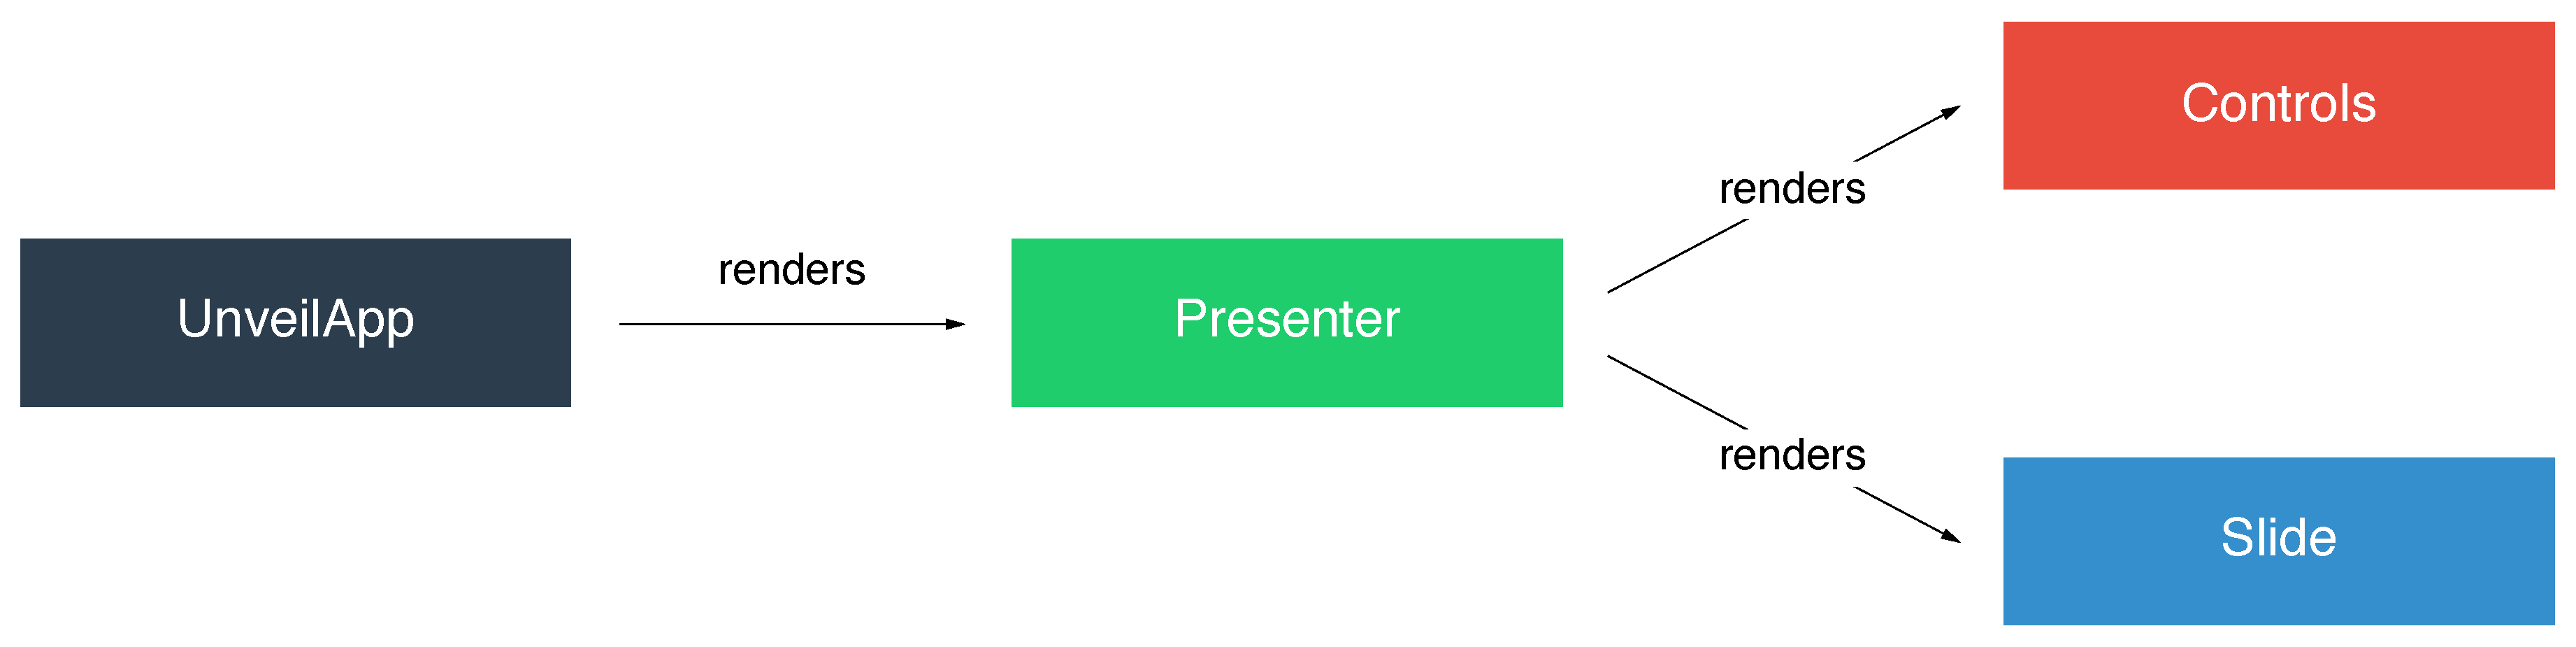
\includegraphics[width=.5\textwidth]{render-pipeline}
\caption{Overview over the render-flow of the application in the extended version of unveil.js. \texttt{UnveilApp} renders the presenter, which then takes care of rendering the (current) slide and all controls.}
\label{fig:implementation-unveil-render-pipeline}
\end{figure}

Another adaption in \texttt{UnveilApp} is the introduction of the \texttt{context} object: Additionally to state and properties, there is a third way of communicating between components in React, called \emph{context}. Instead of having to pass properties from one nested component to the other, every child component can access the context of its parents. The navigator, needed in the controls, was formerly passed from \texttt{UnveilApp} to the controls through several layers. Using context, \texttt{UnveilApp} now defines a number of different variables which are available through context, including current slide and router state, navigator, mode and the state subject discussed in the last paragraph. This makes it easy for new controls and presenters to access the data they need without other layers knowing about them or having to define them.
This adaption was partly due to a change in the render hierarchy: Formerly, \texttt{UnveilApp} itself rendered the presenter (which rendered the current slide) and the controls. However, the presenter needs to be able to also control the rendering of controls (see figure \ref{fig:implementation-unveil-render-pipeline}), adding another layer between the rendering of controls and \texttt{UnveilApp}.

Another part that was added to the unveil.js base library is the \texttt{Notes} component. It allows adding speaker notes to each slide (see program \ref{prog:implementation-technologies-react}). These, however, are not rendered by the slide, but by the presenter, as will be shown in section \ref{sec:implementation-interactive}. One more important new feature is the possibility to configure the next slide in a certain direction (left/right/up/down) and therefore allow for jumping into different branches of the presentation, thus making a presentation even more interactive. The following code, for example
%
\begin{JsCode}
  <Slide name="start" left={[0]}>
    ...
  </Slide>
\end{JsCode}
%
means a navigation \emph{left} (left arrow key pressed, swipe left etc.) will not go to the previous slide defined in the slide-tree, but rather jump to the first slide (of index $0$).


\section{Network Synchronisation Layer}
\label{sec:implementation-network-sync}
% Mention problems with socket io here! --> Corporate firewalls can block socket io entirely, etc.
As mentioned before, the network synchronisation layer is responsible for the communcation between server and client using web sockets. These are created with socket.io, a library which also provides fallbacks for browsers that do not support web sockets yet. However, this library also has a few drawbacks, especially when it comes to corporate networks. As Rob Britton describes in \cite{socketio-problems}, socket.io seems to have problems getting through firewalls and can be blocked by some anti virus software.
Because mobile browser support is essential for this project, I decided to still use this library.

The setup of the socket is simple: one helper function, called \texttt{createSocket} is called in the main entry point of the application to configure which server to connect to:
%
\begin{JsCode}
import { createSocket } from 'unveil-network-sync'
createSocket('46.101.166.172:9000')
\end{JsCode}
%
This function creates the socket and returns it as a singleton, so every component uses the same connection. To make importing even easier, there is another helper, called \texttt{SocketIO} which dan be importet directly and internally calls \texttt{createSocket} to retrieve the singleton:
%
\begin{JsCode}
import { SocketIO } from 'unveil-network-sync'
\end{JsCode}
%

These sockets can then be used to listen to events or to emit them (see program \ref{prog:implementation-network-sync-navigation-receiver}) Like the state subject events, the socket.io events used in this library follow the naming convention of scoping the object targeted in by the event separated by slashes, followed by a colon and the name of the action, e.g. \texttt{state:change} or \texttt{state/slide/voting:start}.

\begin{program}
\caption{Shortened version of \texttt{NavigationReceiver}. First the inherited context properties are set up, then an observable waiting for \texttt{state:change} events from the socket is created. If the incoming request is not the currently displayed slide, the navigator will be pushed a new value.}
\label{prog:implementation-network-sync-navigation-receiver}
\begin{JsCode}
// imports...

export default class NavigationReceiver extends React.Component {
  static contextTypes = {
    navigator:   React.PropTypes.object.isRequired,
    routerState: React.PropTypes.object.isRequired
  }

  componentDidMount () {
    this.observable = Observable.fromEvent(SocketIO, 'state:change')
      .filter((e) => !this.context.routerState.indices.equals(e))
      .subscribe(this.props.navigator.next)
  }
  ...
}
\end{JsCode}
\end{program}
%
The second responisbilty of this library is synchronising the navigation state of the presentation between speaker and audience. To do this, two controls, \texttt{NavigationSender} and \texttt{NavigationReceiver} were implemented. As the names already say, the sender broadcasts the state update, while the receiver is waiting for state updates and starts the navigation process. The latter is used in all modes (default, speaker and projector), whereas the sender is only added to the speaker mode. To make sure the sender does not end up in an infinite loop of sending and receiving its own state changes, the last received state is stored and only navigation events going to a different slide are processed further.

This mechanism, though relatively simple, already enables the audience to follow the presentation, the speaker to use his/her phone as a remote control and any number of projectors to be controlled by the speaker.

\section{Interactive Extension}
\label{sec:implementation-interactive}
The interactive library includes several parts which will be discussed here: a speaker presenter (section \ref{sec:implementation-interactive-speaker-presenter}) as well as different components connected to sharing media (section \ref{sec:implementation-interactive-media}) and voting (section \ref{sec:implementation-interactive-voting}). Additionally controls handling the \texttt{state:initial} event were implemented to redirect new listeners to the current slide in the presentation.

\subsection{Speaker Presenter}
\label{sec:implementation-interactive-speaker-presenter}

The speaker presenter, like the normal presenter, is responsible for rendering controls and slides. In speaker mode, where this presenter is used, notes as well as the upcoming slides (right and down) are also shown (see figure \ref{fig:implementation-interactive-speaker-presenter}).
This means the presenter has to find these next slides, using the router's information about the navigatable directions, and render them in a designated area. To make the presenter view usable on mobile devices, special attention was paid to mobile stylesheets (see figure \ref{fig:implementation-interactive-mobile} (b)). This ensures that everything is big enough to be readable and all buttons are clickable.

\begin{figure}
\centering
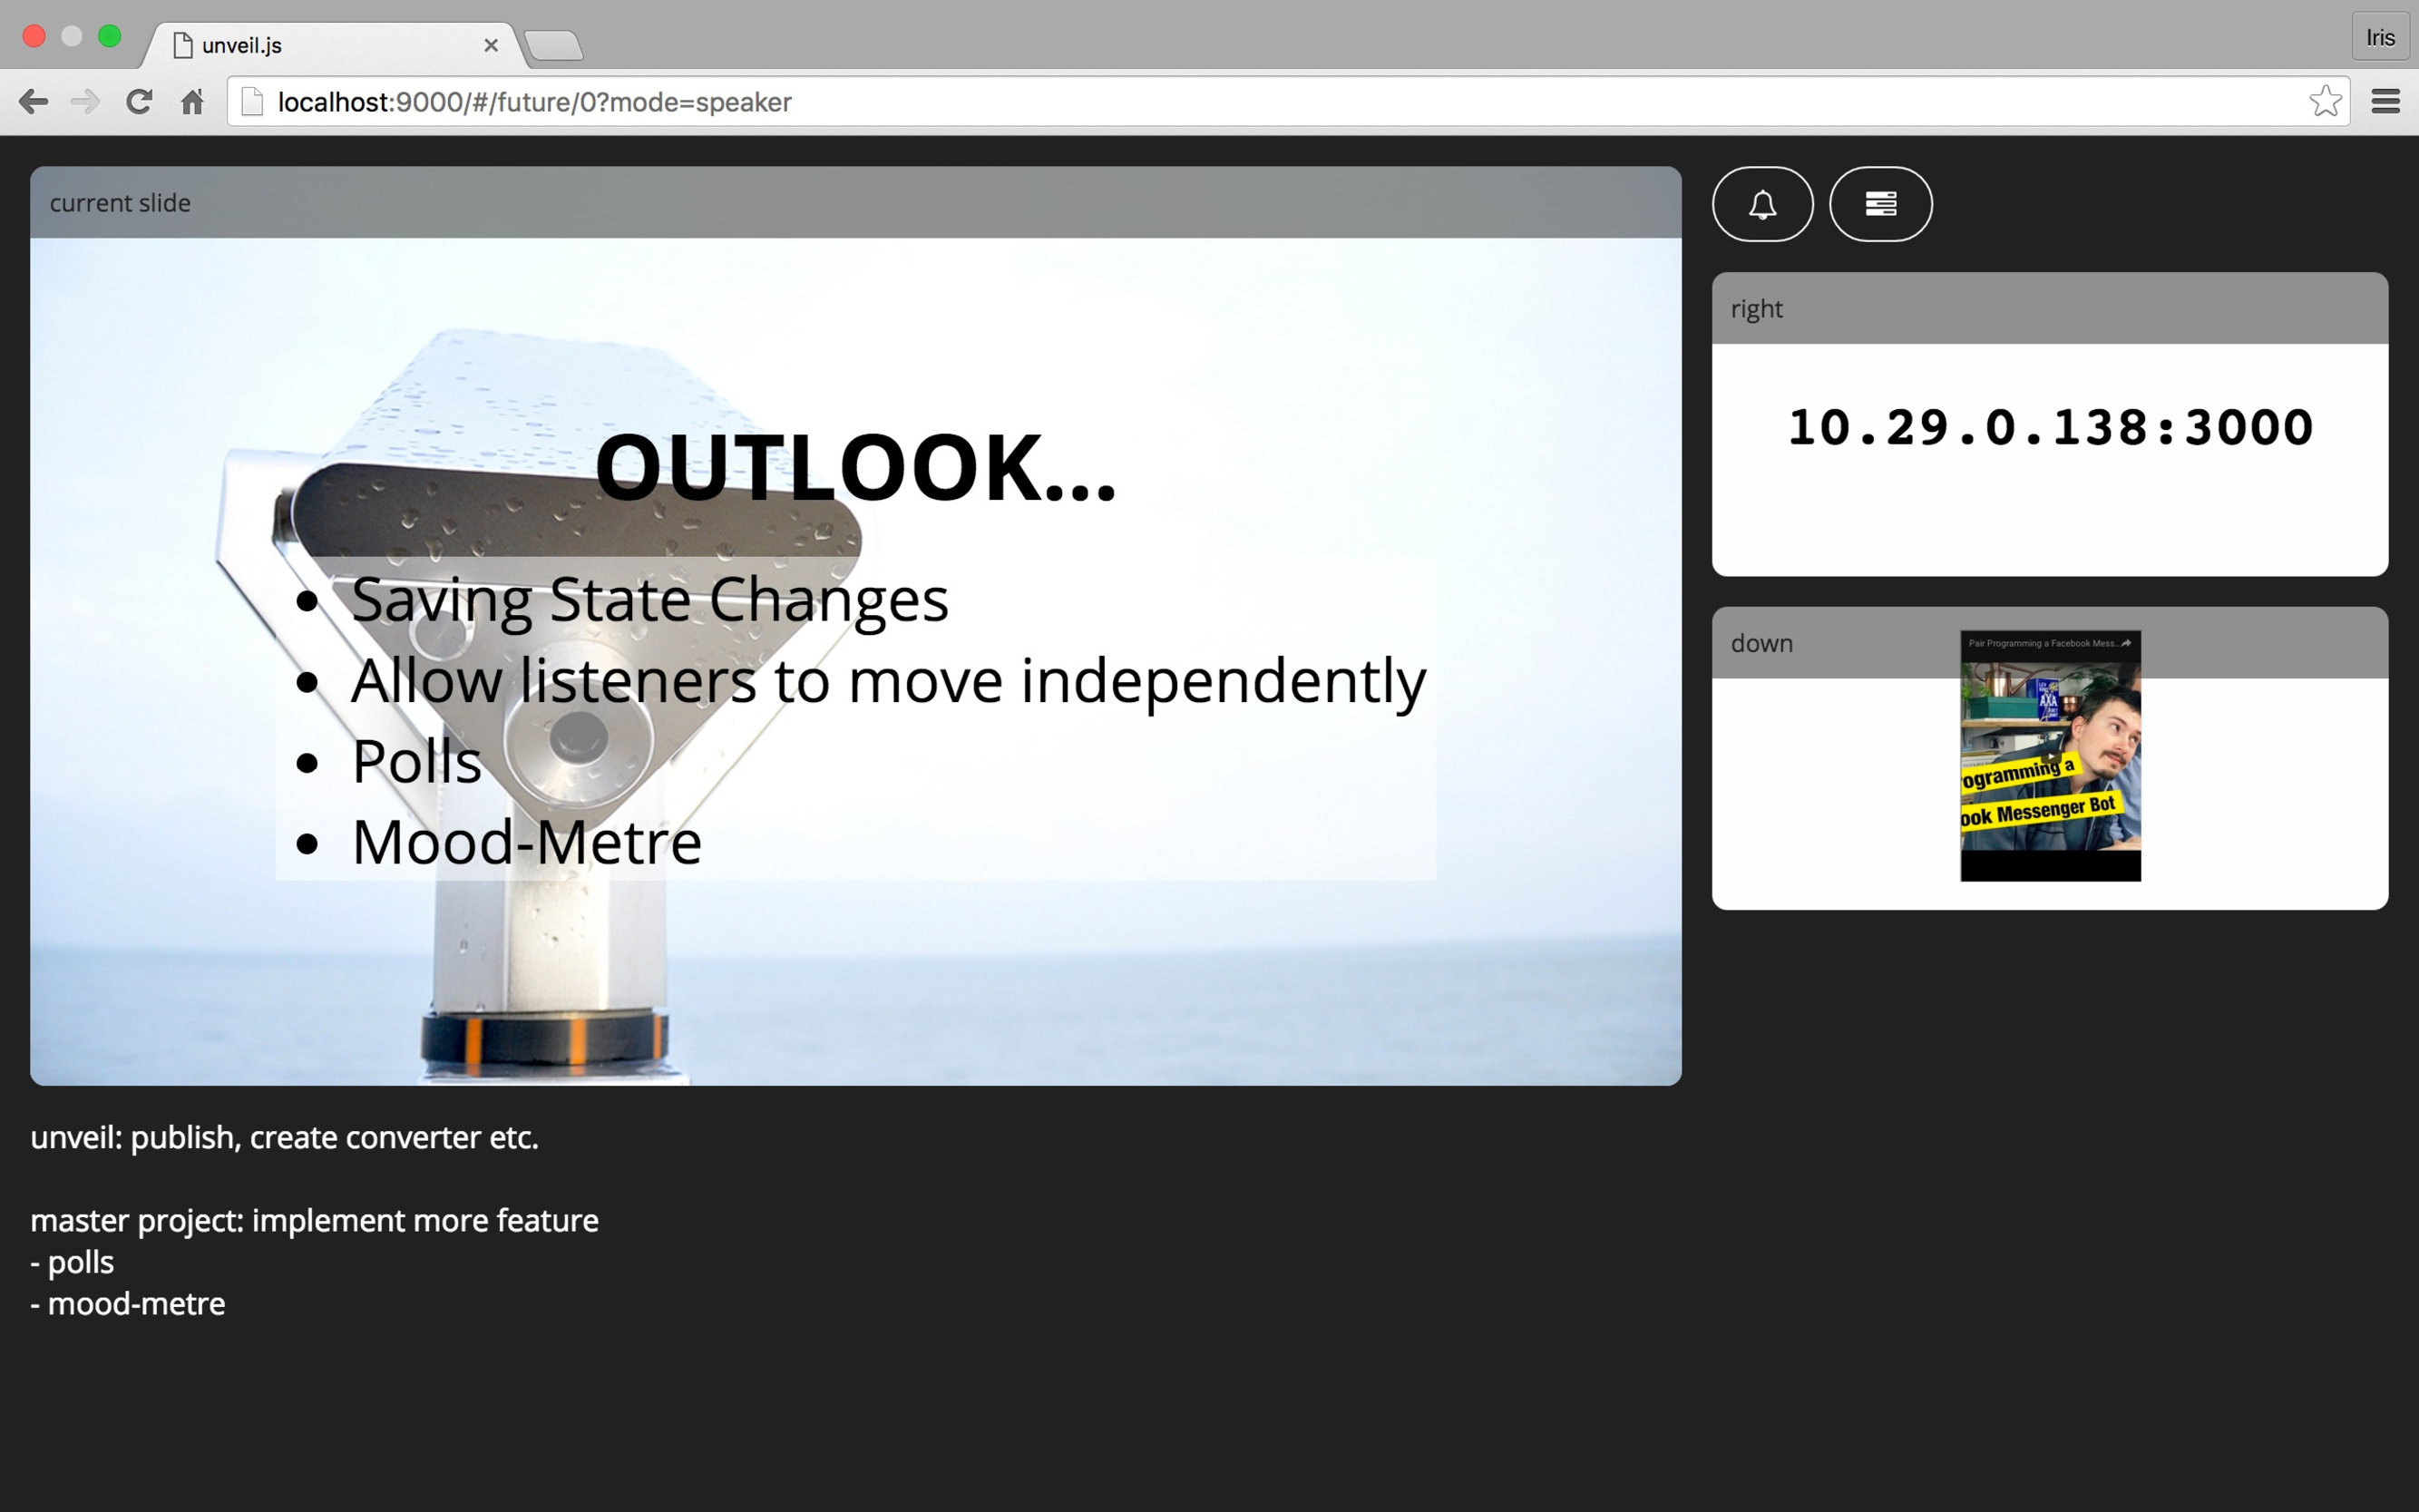
\includegraphics[width=.65\textwidth]{media-accepted-screenshot}
\caption{Screenshot of the speaker presenter with the current main slide, the upcoming slide to the right, available actions (muting and adding votings) and speaker notes.}
\label{fig:implementation-interactive-speaker-presenter}
\end{figure}

\begin{figure}
\centering\small
\begin{tabular}{cccc}
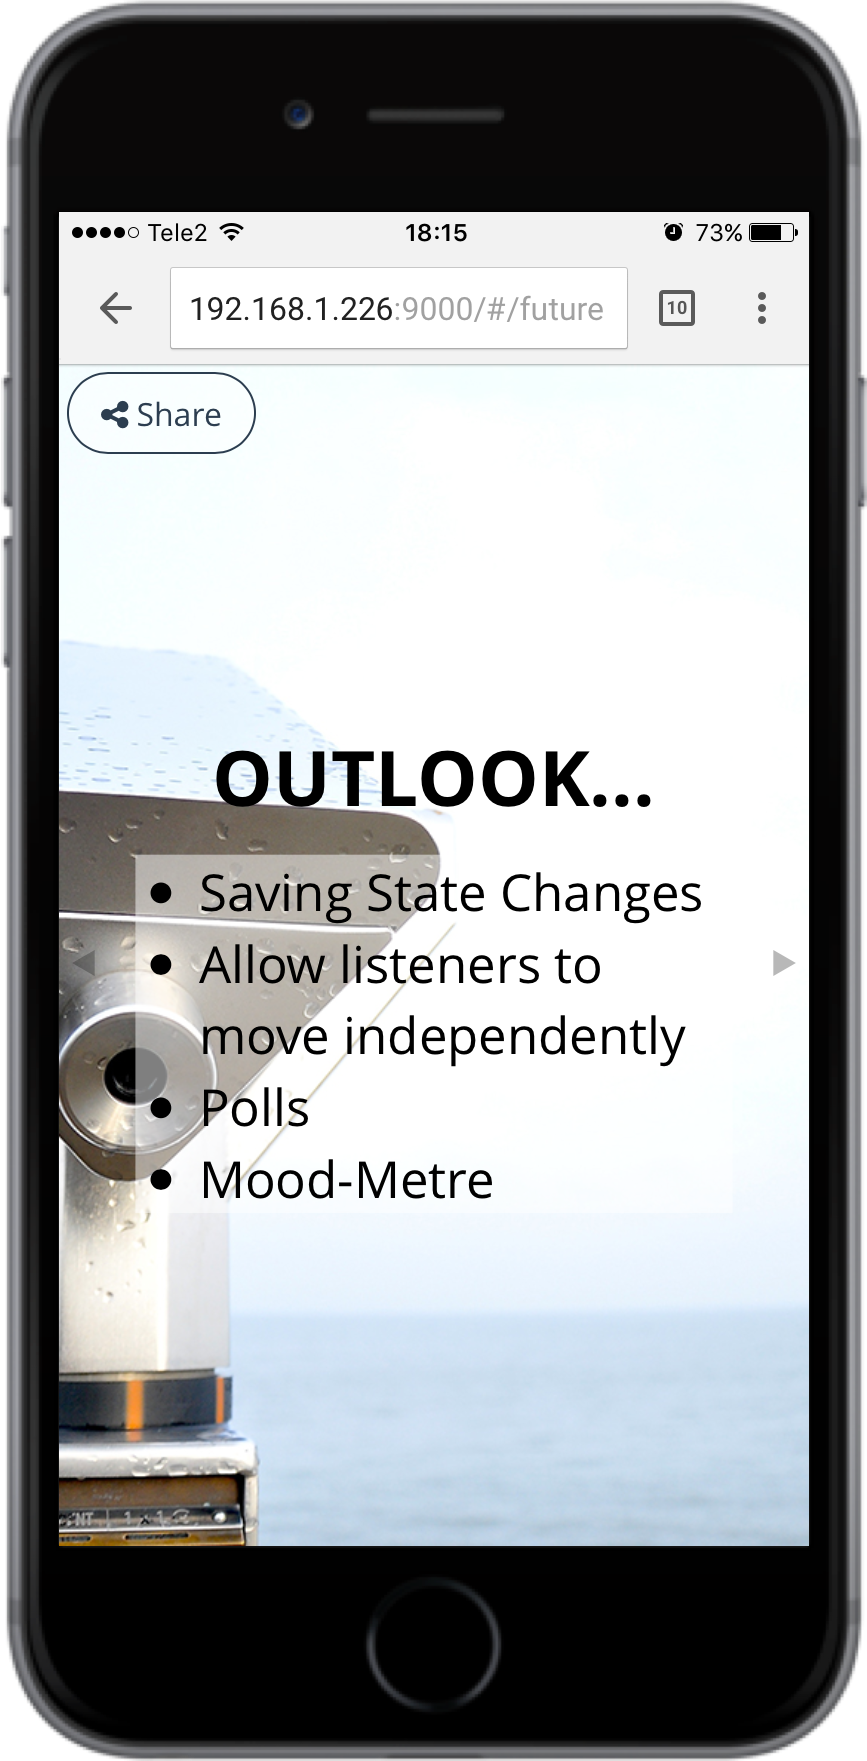
\includegraphics[width=.2\textwidth]{presentation-screenshot-mobile} &
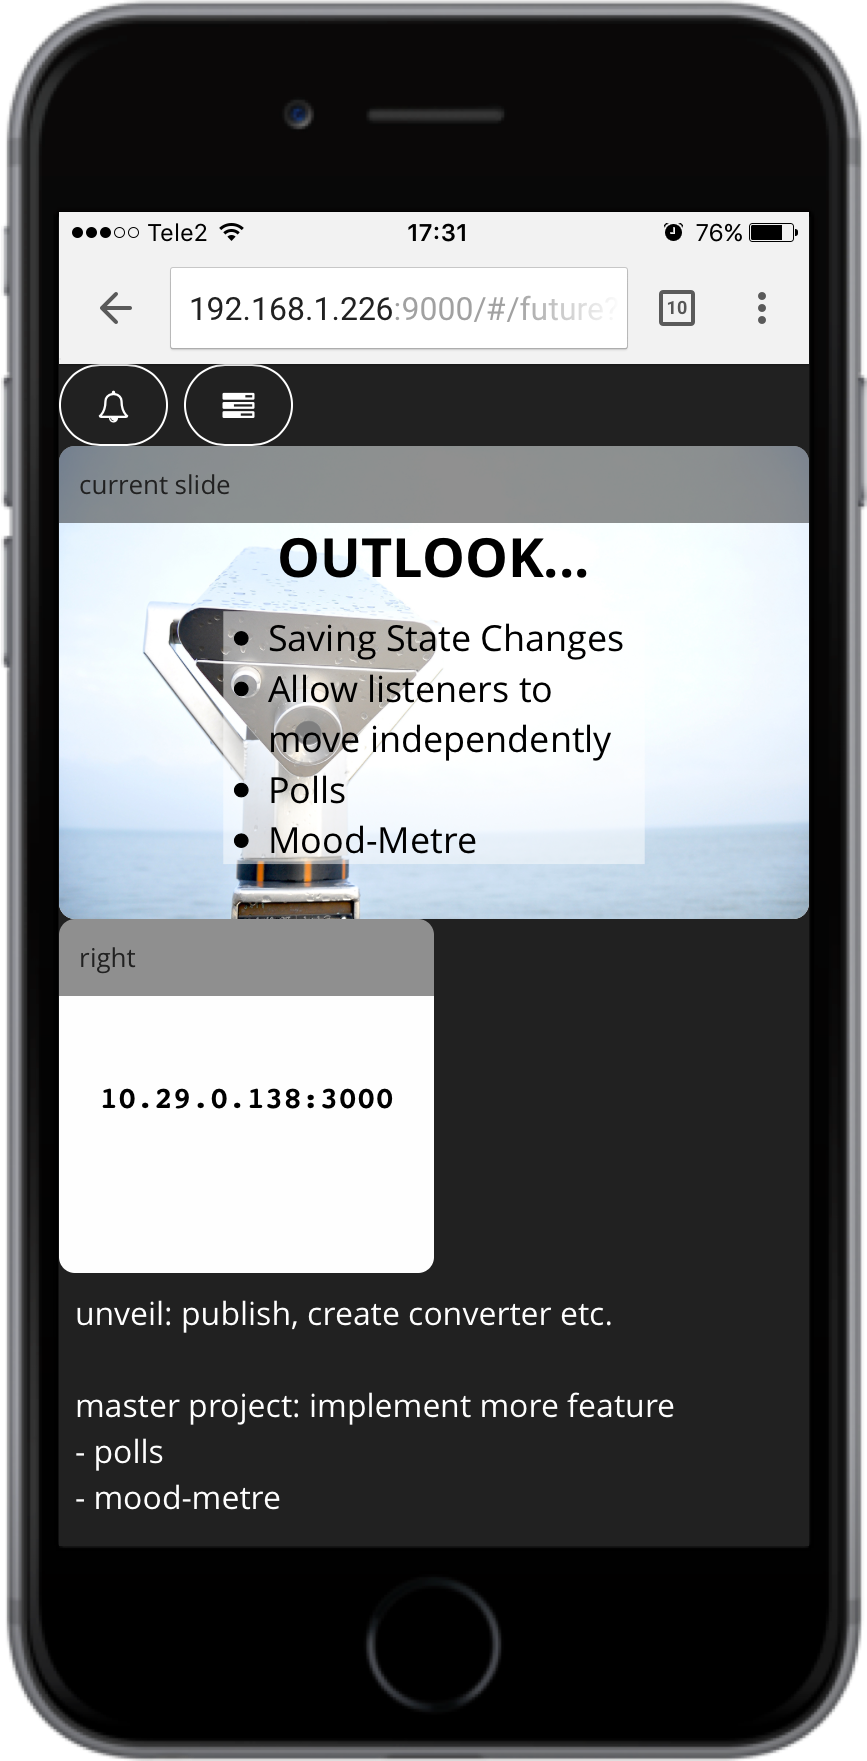
\includegraphics[width=.2\textwidth]{speaker-presenter-screenshot-mobile} &
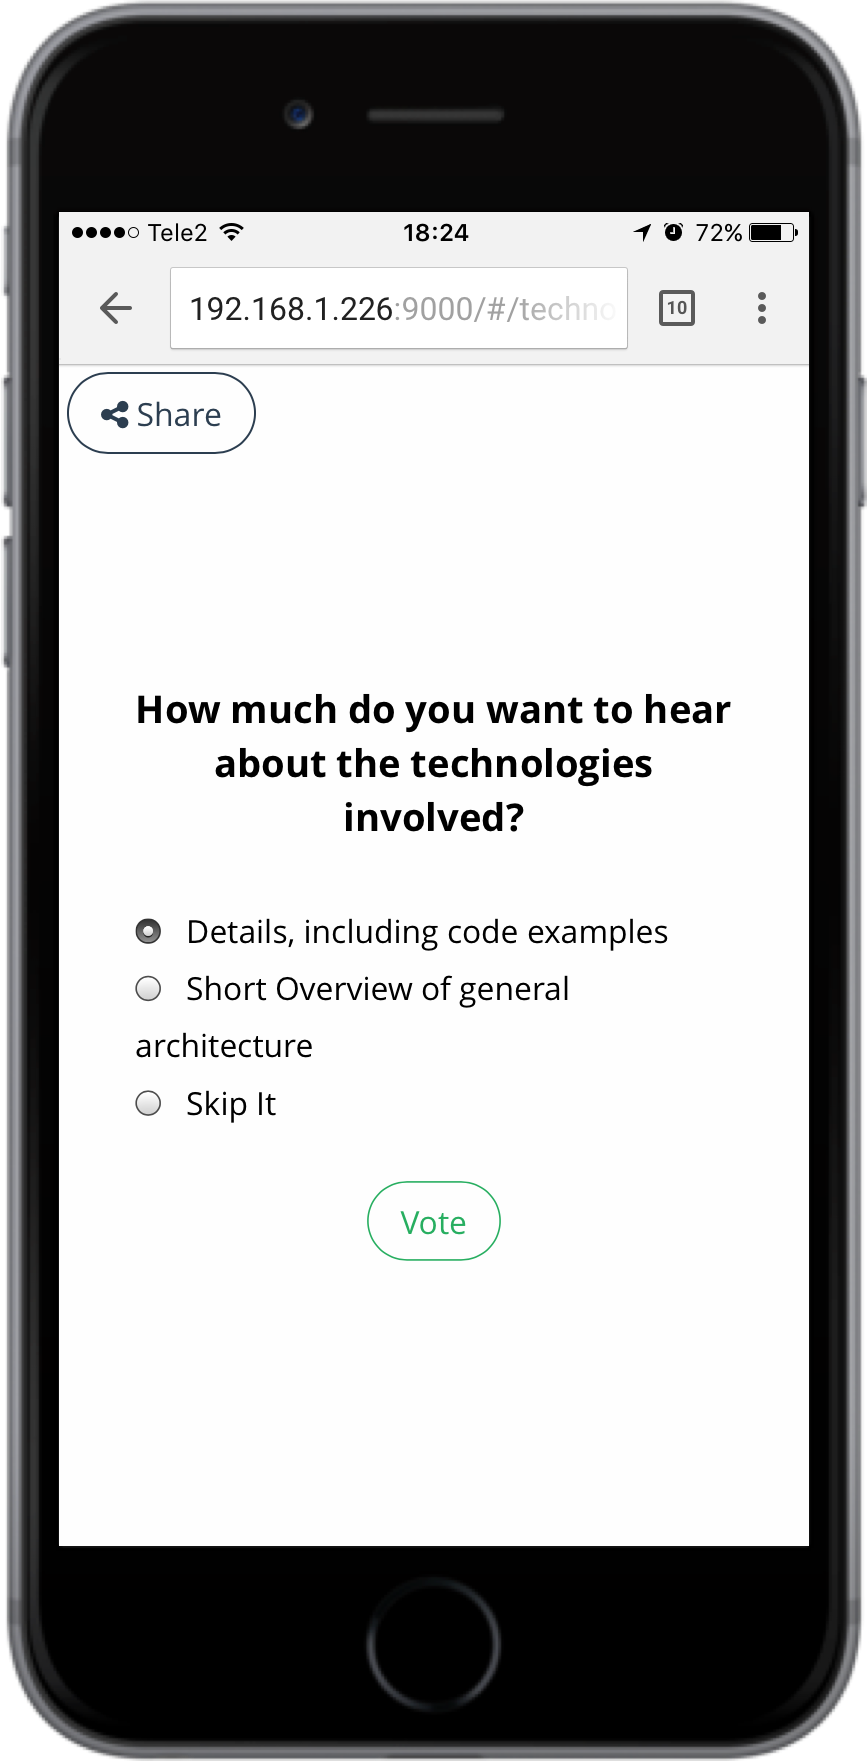
\includegraphics[width=.2\textwidth]{voting-screenshot-mobile} &
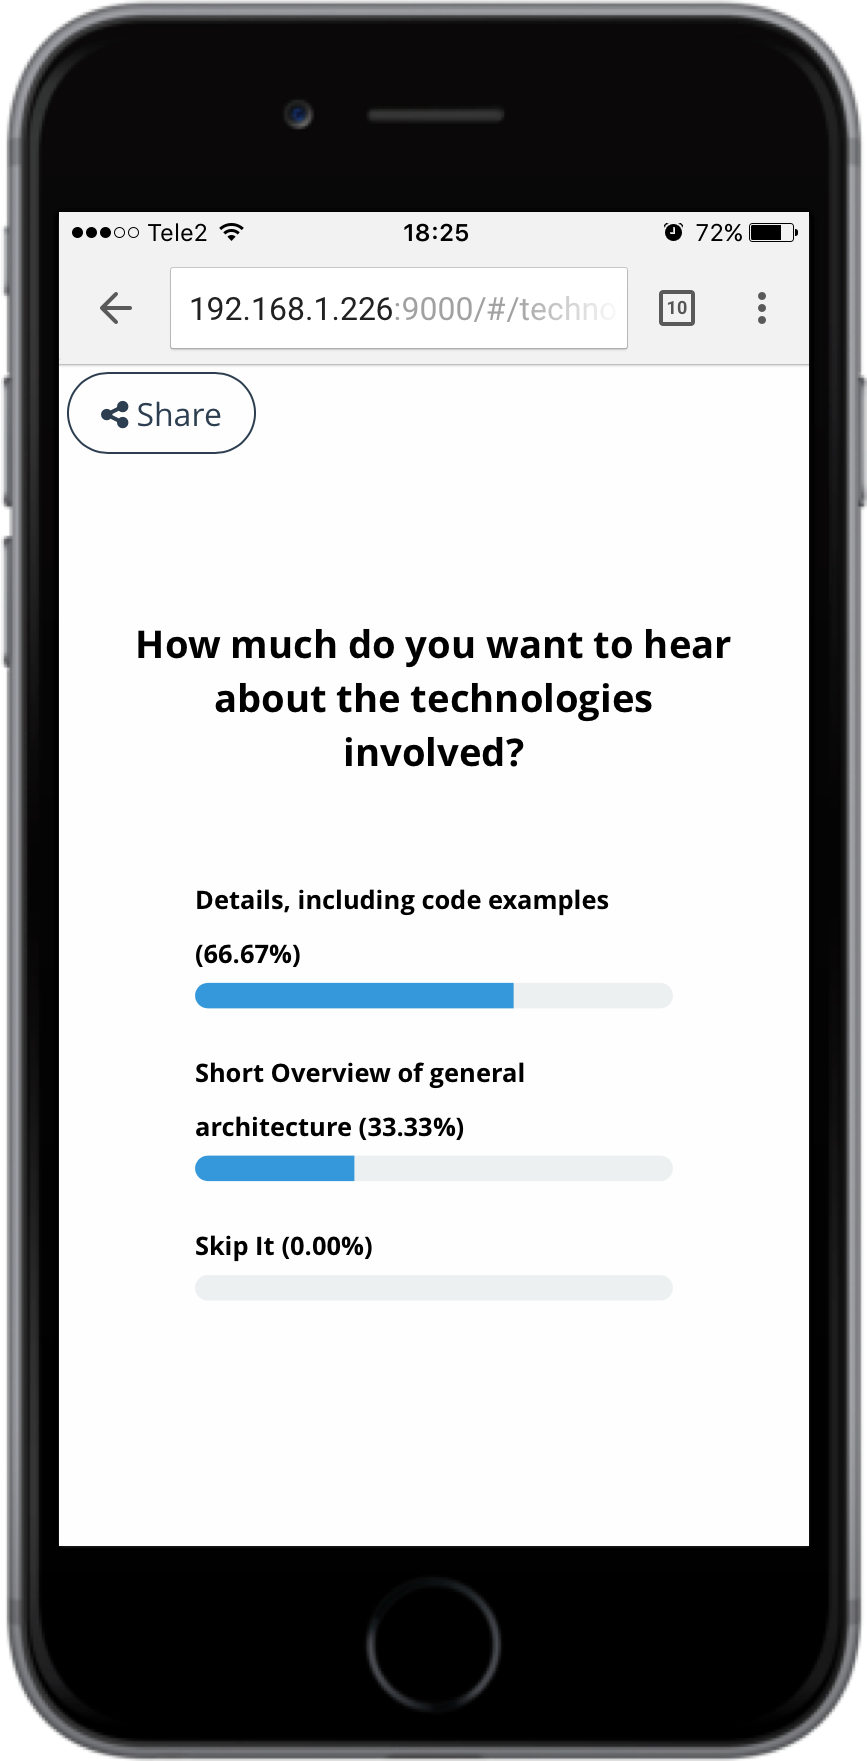
\includegraphics[width=.2\textwidth]{voting-results-screenshot-mobile} \\
(a) & (b) & (c) & (d)
\end{tabular}
\caption{Mobile view of a presentation slide in (a) default mode and (b) speaker mode as well as (c) voting view before voting and (d) voting view after voting. Mind the share button in the left upper corner in (a) as well as the buttons to mute content requests and create votings in (b).}
\label{fig:implementation-interactive-mobile}
\end{figure}

\subsection{Media}
\label{sec:implementation-interactive-media}
Another responsibility of the interactive extension is the possibility for audience members to share content with the presentation. For this to work, three different controls were created: \texttt{MediaSender}, \texttt{MediaReceiver} and \texttt{MediaAcceptor}. The sender is used in the default mode so users can share their content (see figure \ref{fig:implementation-interactive-media} (a)), the acceptor is enabled in speaker mode, to accept or reject incoming media (see figure \ref{fig:implementation-interactive-media} (b)) and the receiver in the end handles the creation of a new slide if the content was accepted and is therefore necessary in all modes. As incoming content requests could disrupt the presentation flow and distract the speaker, an option to mute the requests was built into the application. If the \emph{do not disturb} mode is turned on, slides will silently be added as subslides, without causing the acceptor modal to open. This way the audience' additions can be re-visited after the end of the presentation. Generally, this feature can be used to either post a link to an interesting picture, website or even youtube video, or also as text input, for example to add a comment or a question regarding a certain slide. This works through the introduction of the presentation components \texttt{Media} and \texttt{IFrame}, which, depending on the shared content, render an image-tag, blockquote or IFrame. The differentiation of these is carried out with regular expressions, as the following to check if the content is the link to an image:
\begin{JsCode}
isImg (str) {
  let imgRegex = new RegExp(/\.(jpe?g|png|gif|bmp)$/i)
  return imgRegex.test(str)
}
\end{JsCode}

As far as the implementation of the controls is concerned, these ones are the first ones discussed in the present thesis makeing use of the \texttt{render()} method. It is used to output the \emph{share} button in the left upper corner in default mode (see figure \ref{fig:implementation-interactive-mobile} (a)) as well as the share modal opened when clicking on said button (see figure \ref{fig:implementation-interactive-media} (a)). The same happens in the \texttt{MediaAcceptor}, which uses the \texttt{render()} method to display the \emph{mute} button shown in figure \ref{fig:implementation-interactive-speaker-presenter} as well as the modal for accepting media (see figure \ref{fig:implementation-interactive-media} (b)).

These are also the first controls using state: in the sender a click on the share button sets the state variable \texttt{sharingMode} to \texttt{true} and through that enables the rendering of the modal. In the acceptor an array of \texttt{requests} is filled as new content is shared and emptied again, as the speaker accepts or denies them.

On event level, the socket events \texttt{state/slide/add:accept} and \texttt{state/ slide:add} are included in the process of sharing new content, in the end an unveil state event of type \texttt{state/slide:add} lets \texttt{UnveilApp} create the new slide and add it to the slide tree. The whole flow is outlined in details in figure \ref{fig:implementation-interactive-media-pipeline}.

\begin{figure}
\centering\small
\begin{tabular}{cc}
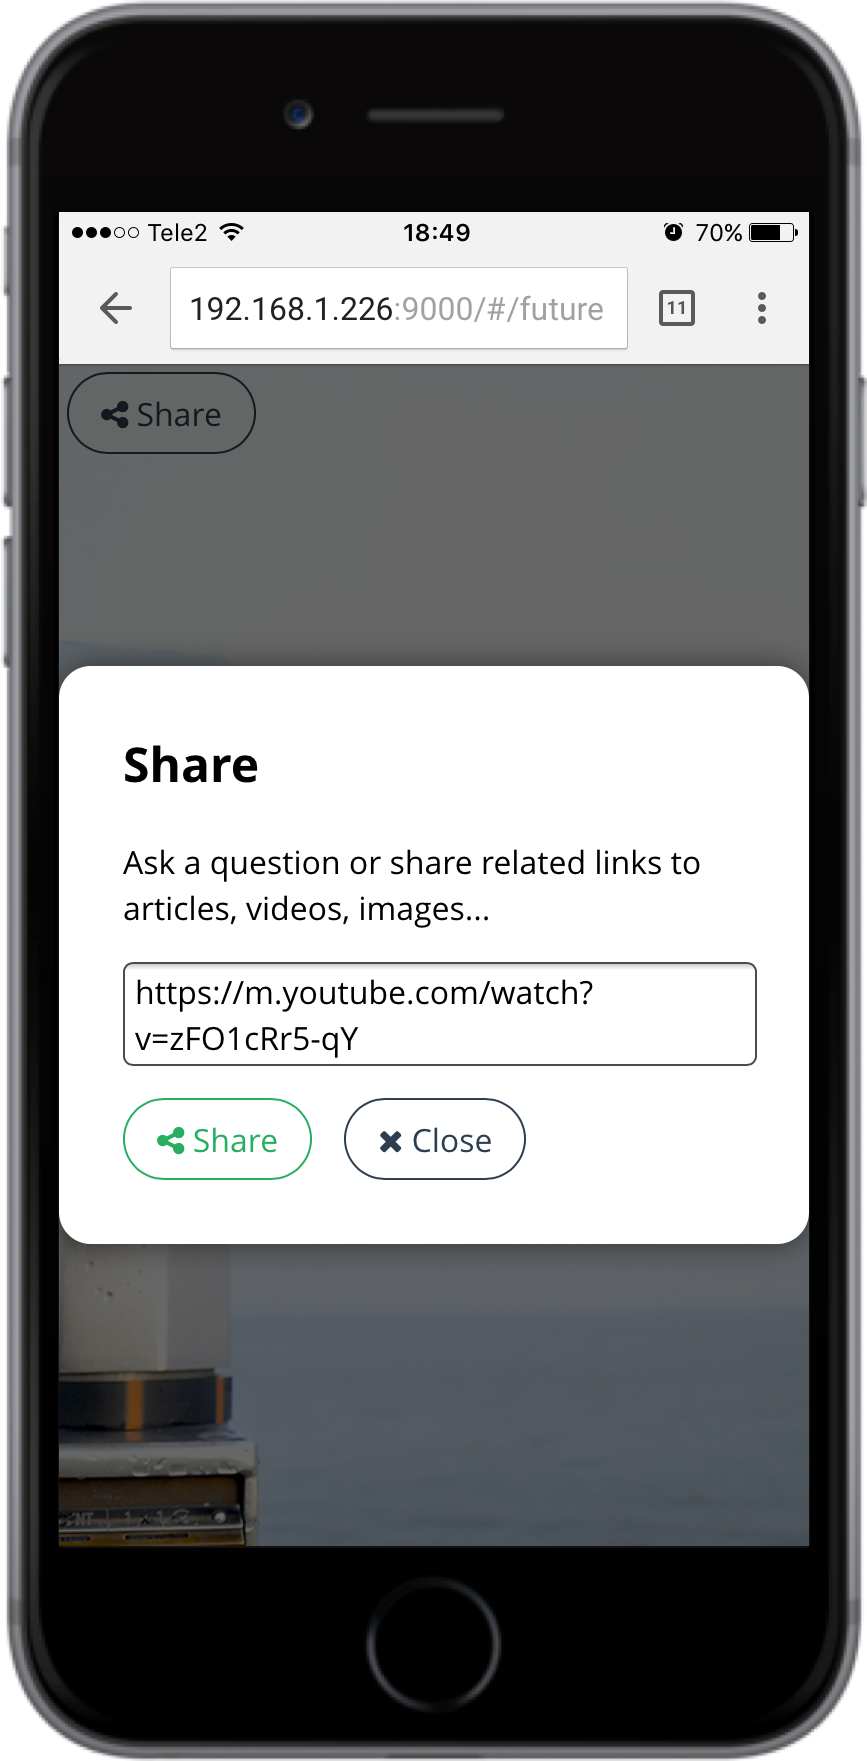
\includegraphics[width=.2\textwidth]{media-screenshot-mobile}
 &
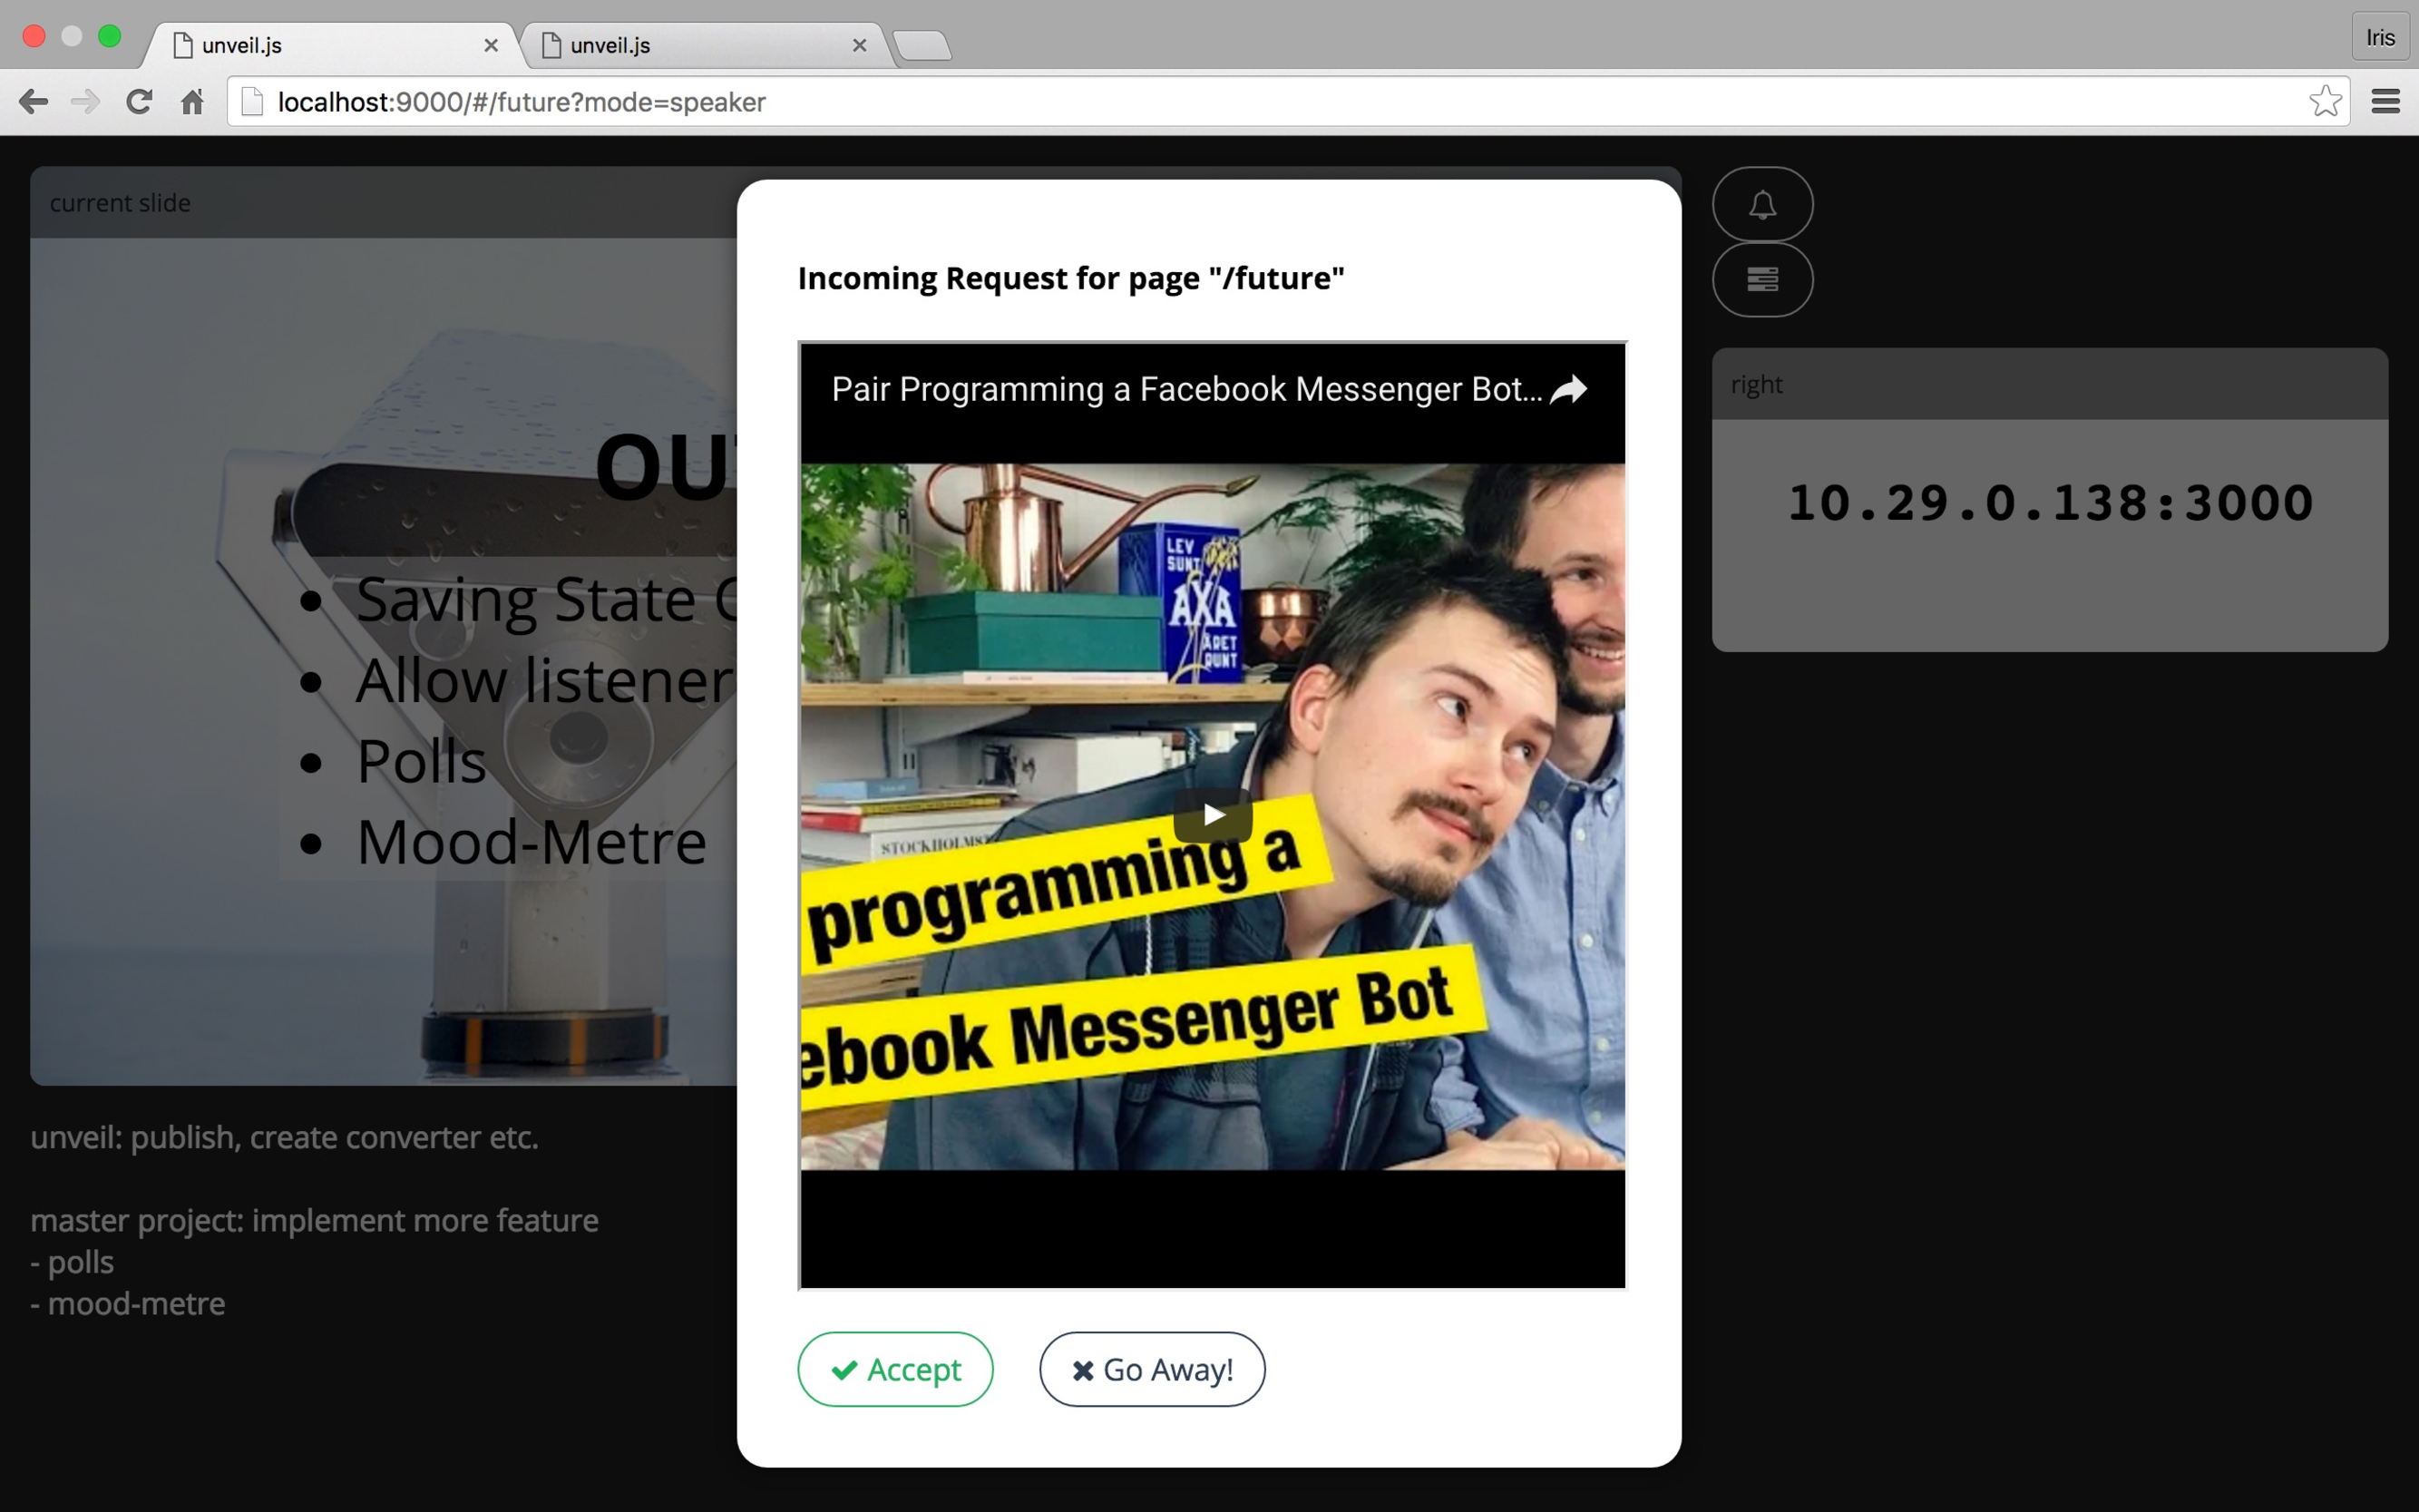
\includegraphics[width=.65\textwidth]{media-acceptor-screenshot} \\
(a) & (b)
\end{tabular}
\caption{Screenshots of sharing content. (a) media sender on mobile phone shares youtube link (b) speaker receives content request.}
\label{fig:implementation-interactive-media}
\end{figure}

\begin{figure}
\centering
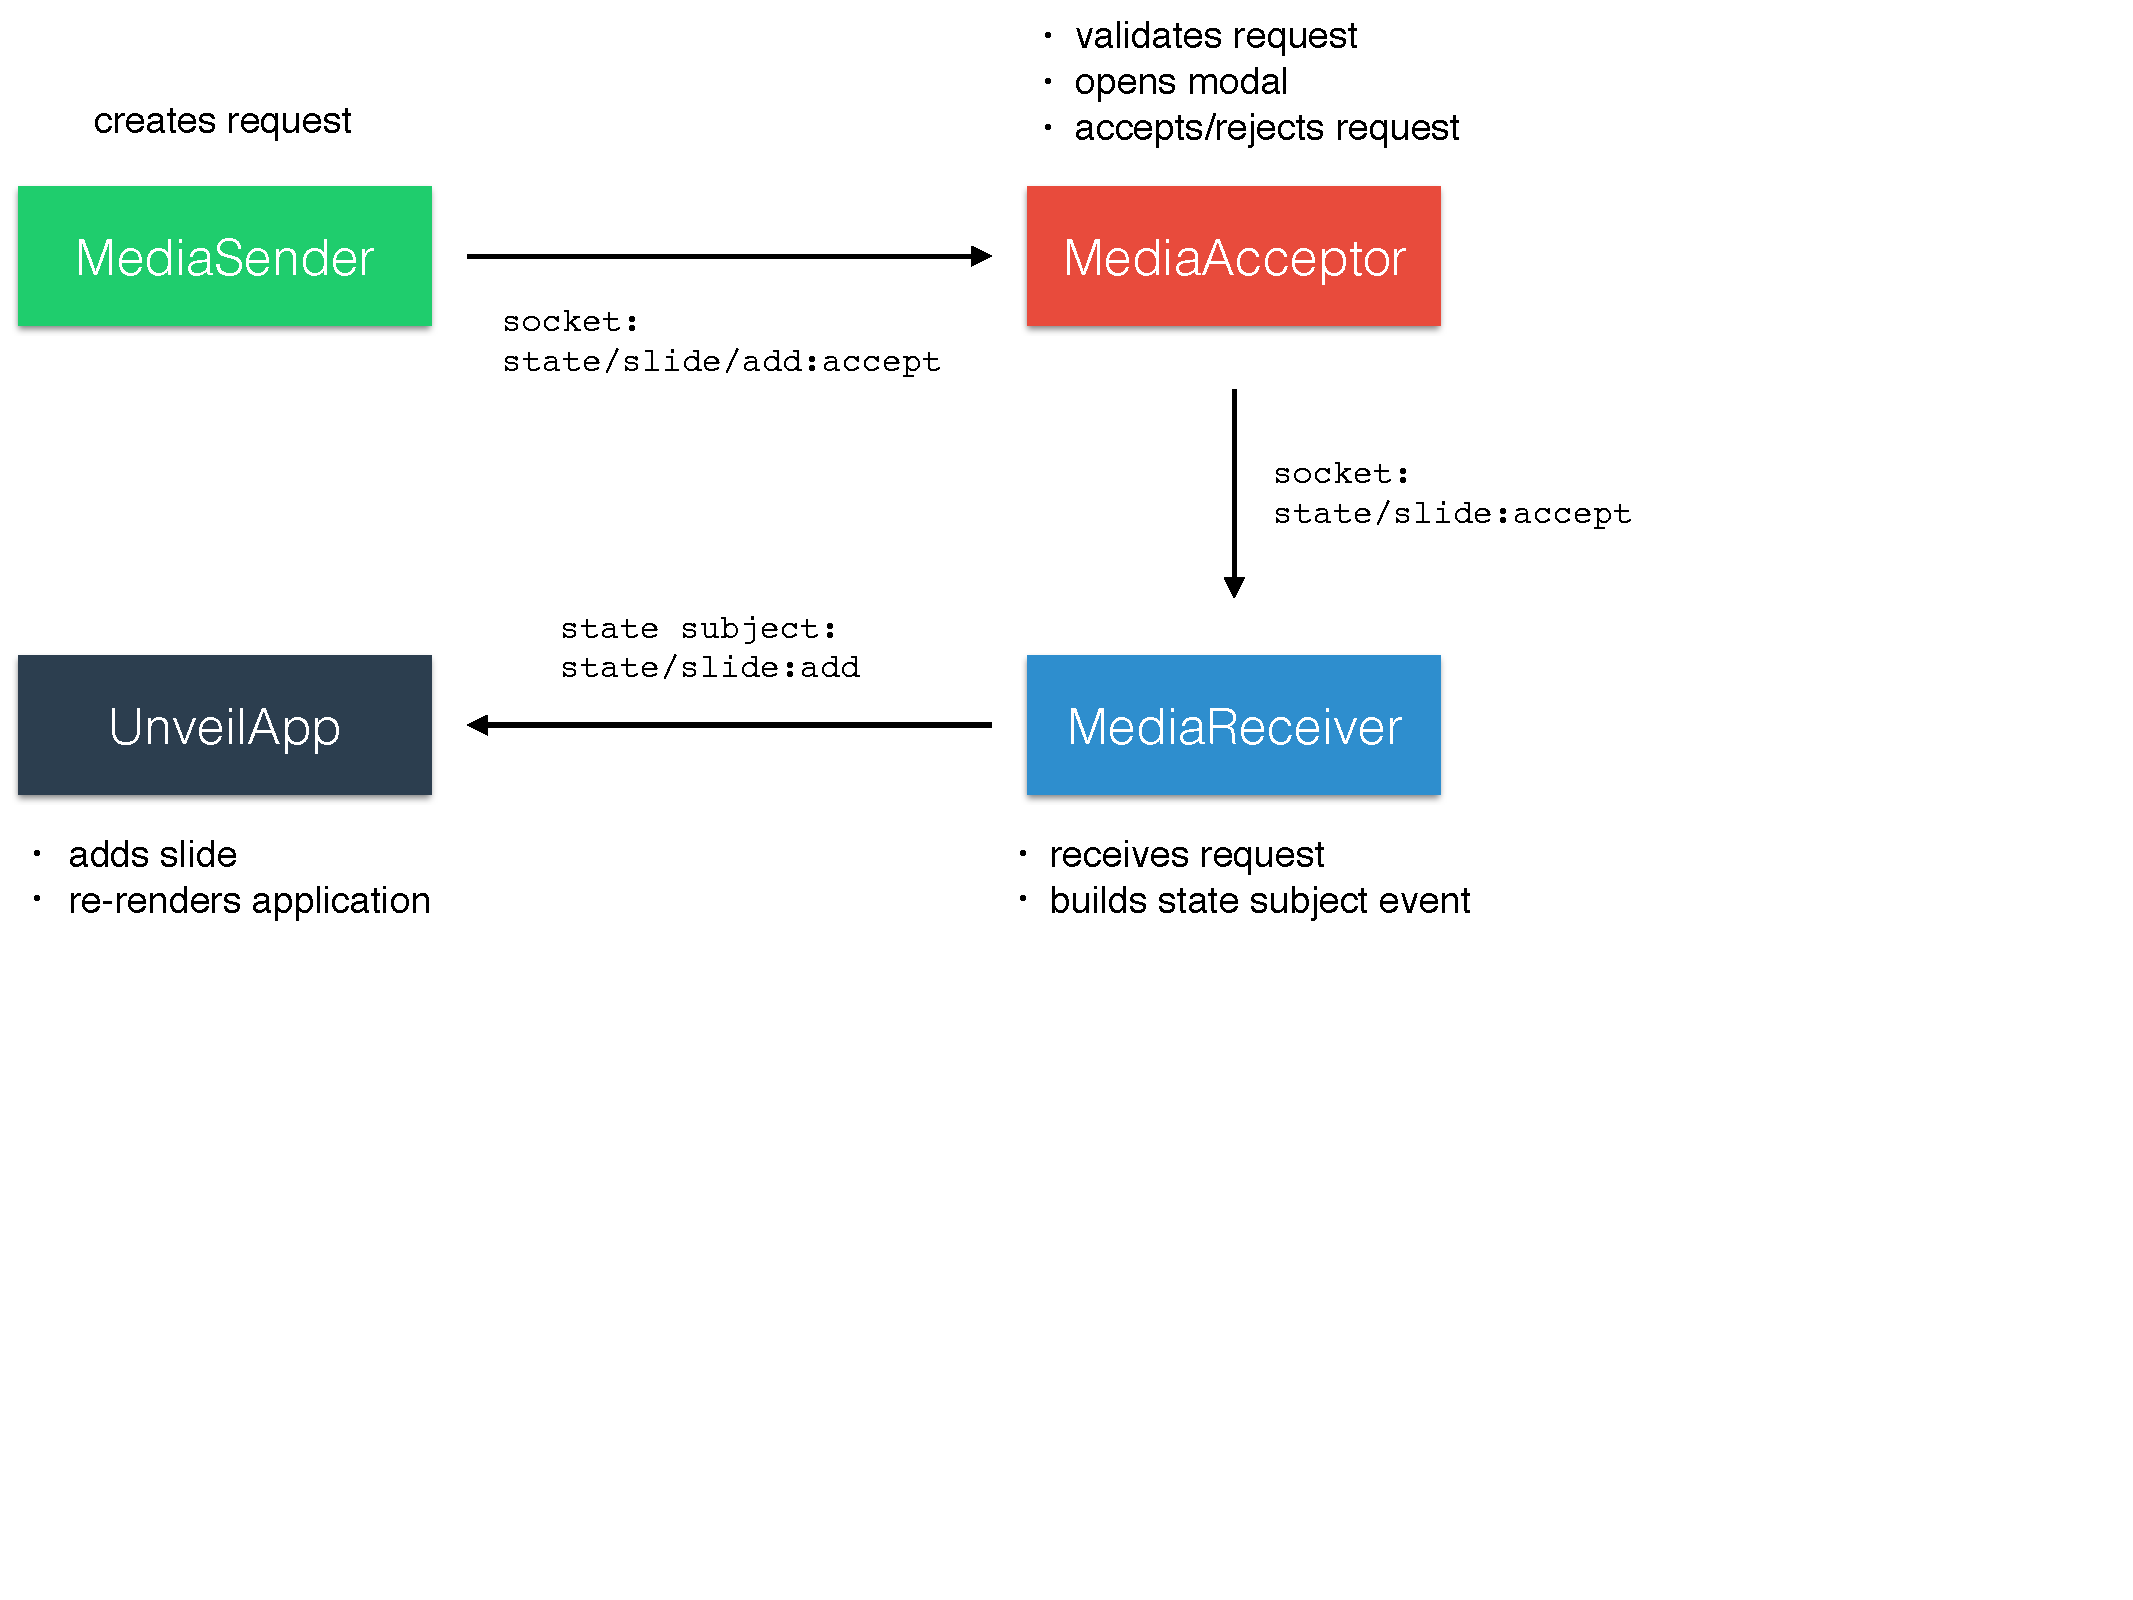
\includegraphics[width=.8\textwidth]{media-pipeline}
\caption{Flow of adding content, monospaced text symbolises type and name of events. First the \texttt{MediaSender} of the default mode sends a request, which the speaker mode's \texttt{MediaAcceptor} listens to. If the request is accepted by the speaker or requests are muted, another socket event is broadcast, which the \texttt{MediaReceiver} waits for. This component is enabled in all modes and emits the state subject event to add a new slide, which \texttt{UnveilApp} reacts to.}
\label{fig:implementation-interactive-media-pipeline}
\end{figure}

\subsection{Voting}
\label{sec:implementation-interactive-voting}

The last group of components connected to the interactive extension covered in this chapter allow speakers to create votings (both during in the preparation of the presentation and on-the-fly as shown in figure \ref{fig:implementation-interactive-voting}) and members of the audience to vote (see figure \ref{fig:implementation-interactive-mobile} (c) and (d)).

\begin{figure}
\centering
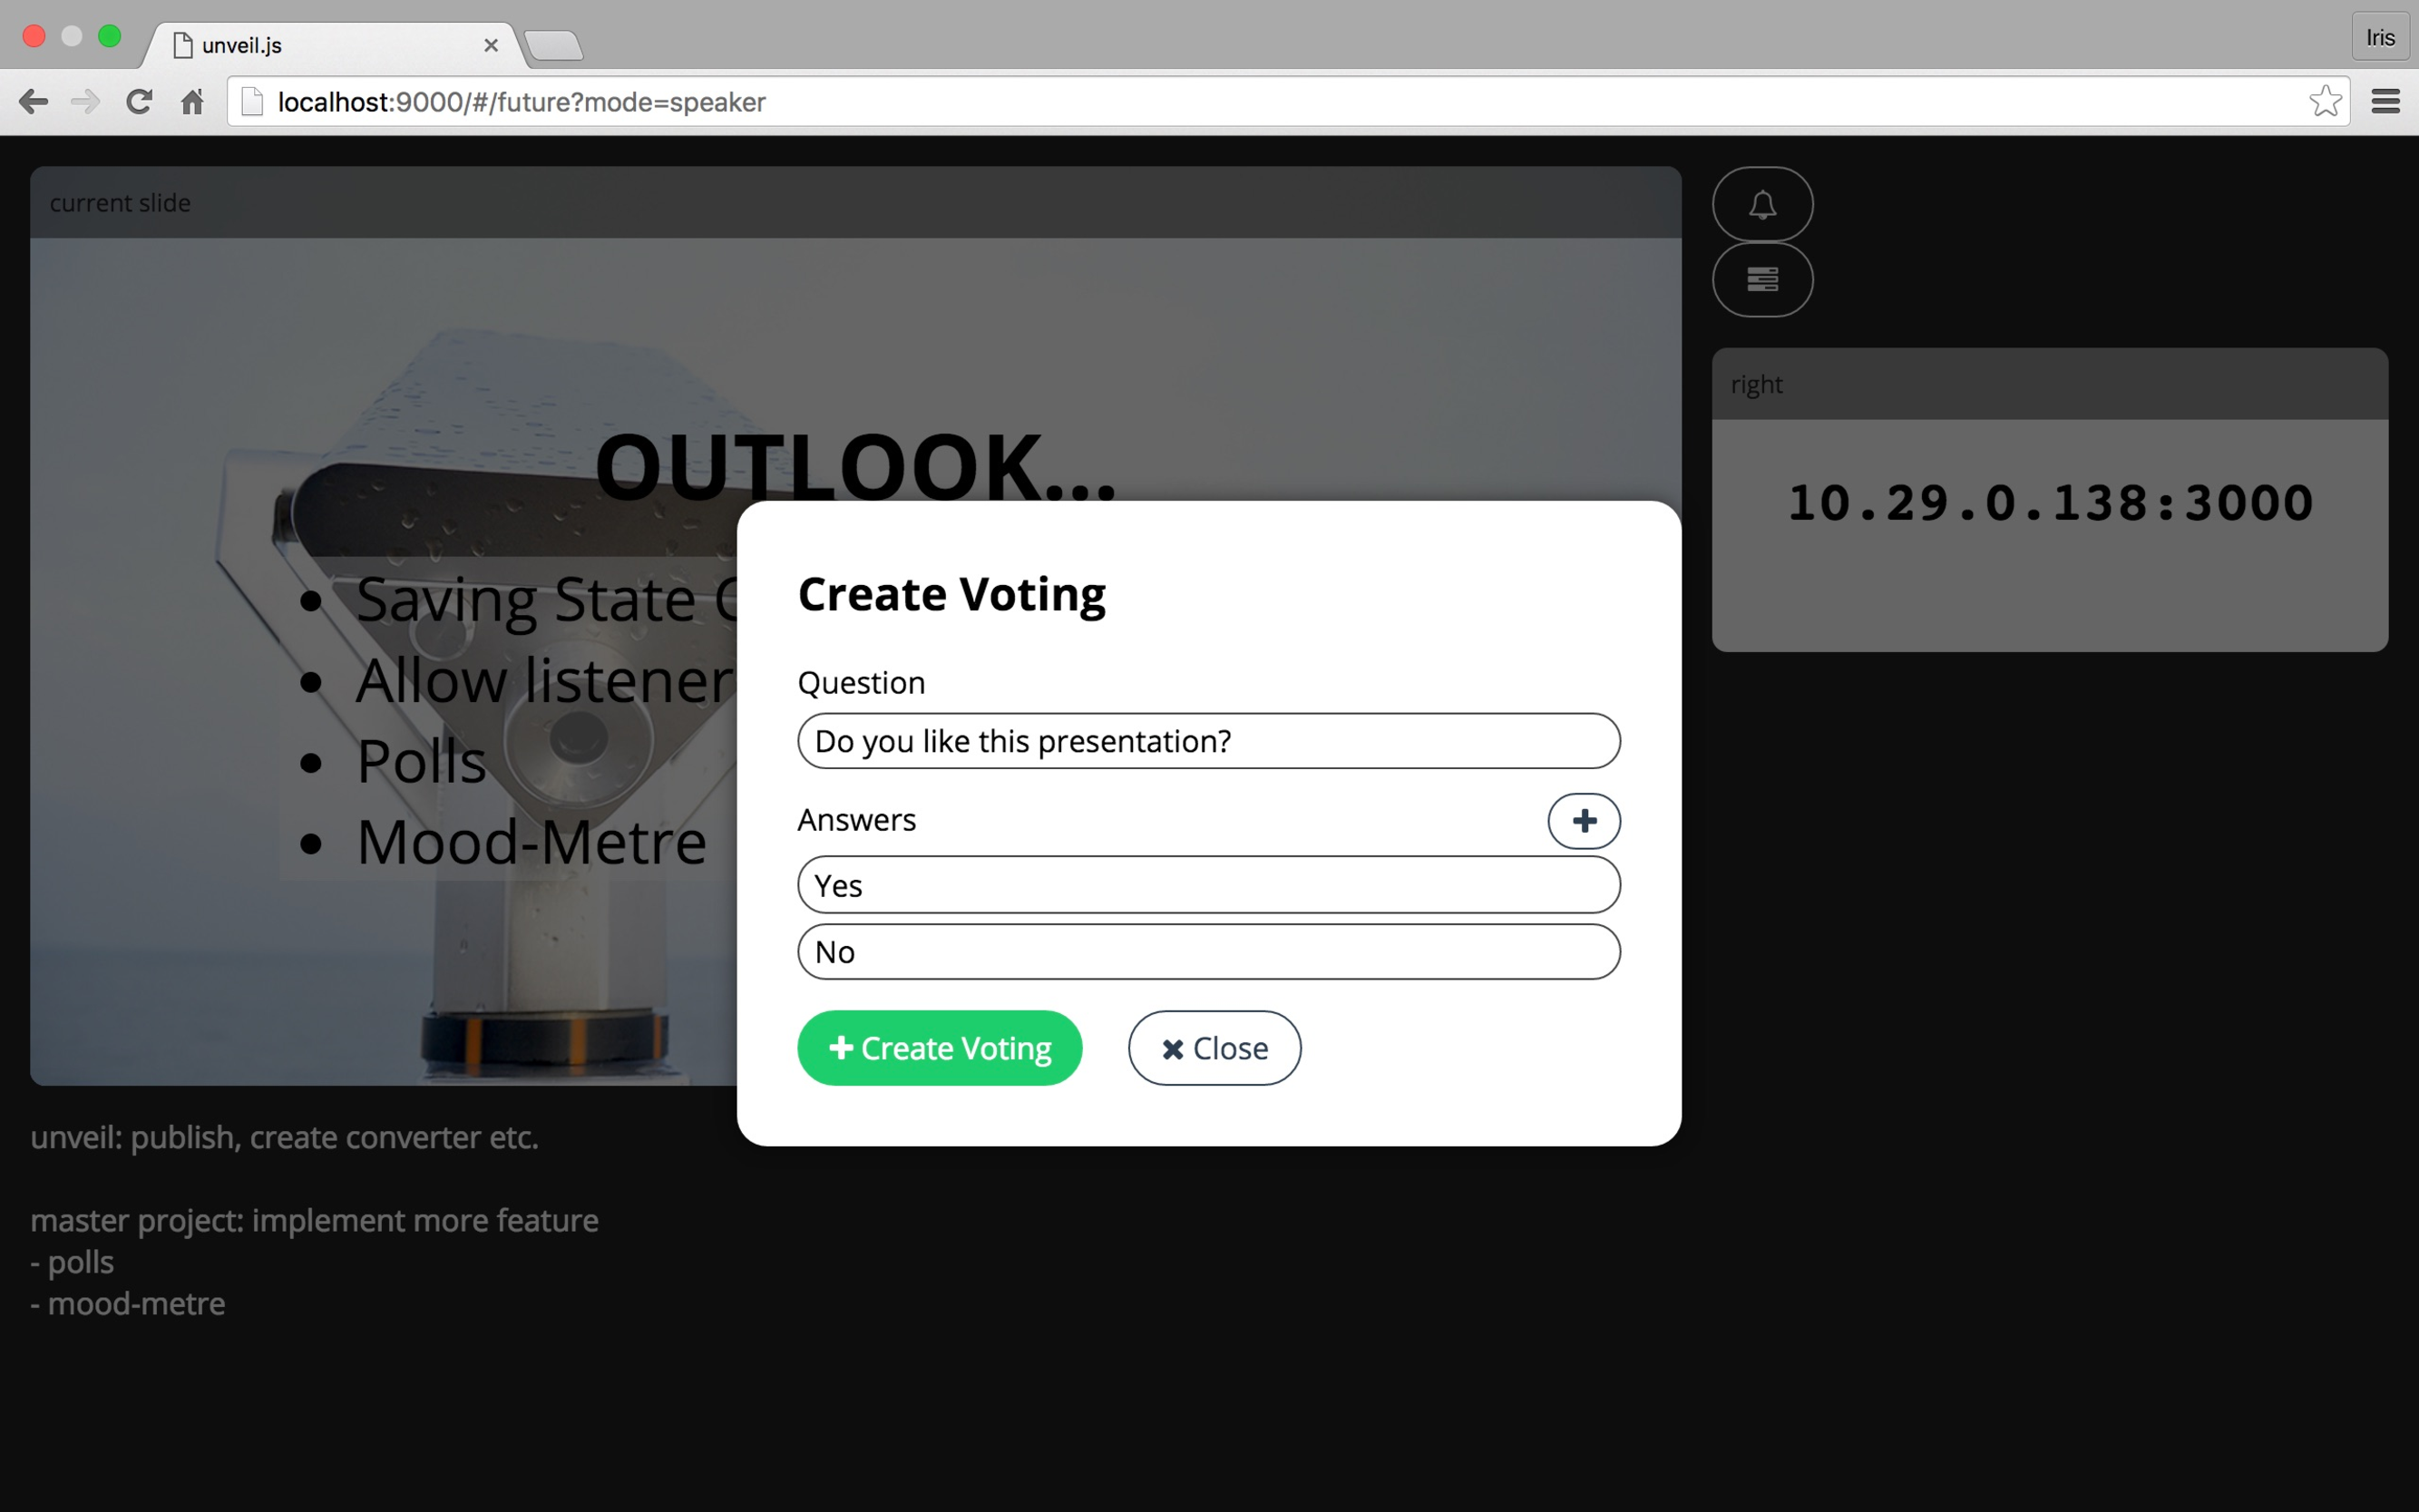
\includegraphics[width=.65\textwidth]{voting-creation-screenshot}
\caption{Screenshot of the desktop speaker mode, creating a new voting, on-the-fly, during a presentation.}
\label{fig:implementation-interactive-voting}
\end{figure}

The main presentational component involved in the voting process is \texttt{Voting}, which keeps track of the current voting scores and has a \texttt{Question} and a number of \texttt{Answer} components as children (see program \ref{prog:implementation-interactive-structure}). \texttt{Voting} also remembers if an audience member has already voted and if so, displays \texttt{Result} components. In speaker and presenter mode only these results are shown.

\begin{program}
\caption{Example code for preparing a slide with voting.}
\label{prog:implementation-interactive-structure}
\begin{JsCode}
<Voting name="like">
  <Question>Do you like these slides?</Question>
  <Answer value="yes">Yes</Answer>
  <Answer value="no">No</Answer>
</Voting>
\end{JsCode}
\end{program}

The audience can start voting as soon as the speaker navigates to the slide with the voting, until then the vote button is disabled. Once the voting has started, the possibility for all audience members to navigate to a different slide is disabled. This happens in the \texttt{VotingNavigatableSetter}, which is only installed for default mode. The voting start event, as well as the voting end event are broadcast by the \texttt{VotingController}, which checks the speaker's current slide for the occurence of a \texttt{Voting}.

Once the voting has started, internally, the \texttt{Voting} component remembers which answer the user has clicked in the \texttt{answer} state variable. Once the submit button is pressed, a \texttt{state/slide/voting:answer} event is fired and broadcast to all clients, which update their internal voting results.
Because the results of the voting should be available throughout the whole presentation and not be reset when leaving the slide, \texttt{Voting} also handles the communication with local storage, to store current results.

\section{Server}
\label{sec:implementation-server}
% shortly talk about server and how any server could really be used for this.
As shortly outlined before, the focus of this project was never the server, but instead the client. For this reason the server was kept as lightweight and \emph{dumb} as possible, only handling the most important communication. In reality, it acts as a proxy and broadcaster between the clients and serves the JavaScript and HTML files. This has the advantage that other developers can use their own servers and technology stacks without relying on the architecture chosen for the example presentation. Literally the only requirement for the server is to support Web Sockets. However, the disadvantage is that currently all state changes are only persisted on the client-side. This is good for testing, as a reset is only a page-reload and clearing of local storage away, but means audience members joining the presentation after any additional slides were added, will not have the same state of the presentation.

The server developed for the project presentation of the Interactive Media course IM690 runs on Node.js, using Express\footnote{\url{http://expressjs.com/}} as a framework. To again emphasise how low the requirements for such a server are, a working example implementation can be found in program \ref{prog:implementation-server-code}. Additionally to this code, the server in the unveil-client-server repository also includes a \texttt{lastState} variable, in which the last navigation state is stored. Every time a new client connects, this state is then emitted with a \texttt{state:initial} event. Moreover, socket.io does not currently support wildcards in events, which is why it was necessary to add the code snippet discussed in \cite{socket-io-wildcards}.

\begin{program}
\caption{Very simple possible implementation of a server running the thesis project with Node.js and Express. \cite{socket-io-wildcards} describes how wildcard support can be added to socket.io.}
\label{prog:implementation-server-code}
\begin{JsCode}
var express = require('express'); var app = express();
var server = require('http').createServer(app);
var io = require('socket.io')(server);

// directory 'client' will be served by server
app.use(express.static(__dirname + '/../client/'));

io.on('connection', function(socket) { // setting up socket io
  socket.on('*', function(event, data) {
    io.emit(event, data);
  });
});

server.listen(9000, function () {
  console.log('Unveil server listening on port 9000!');
});
\end{JsCode}
\end{program}

\section{Example Application}
\label{sec:implementation-client}
% how is everything defined? what has to be included?
% what are the steps of building an application with unveil?
% how are the slides defined? how are they styled? what about the modes?

To conclude this chapter, I want to show how all the discussed libraries in the end can be put together to a presentation. The whole presentation can be found in the unveil-client-server repository.

The first step to use unveil.js and its extensions is to start a new project, require the necessary npm packages and set up an \texttt{index.html} page which includes the necessary stylesheets and scripts.
The entry point for these scripts is the file \texttt{index.js}, in which the whole presentation is set up and unveil.js is configured by setting up its modes (see program \ref{prog:implementation-client-modes}). As explained before, slides are defined in HTML using the components unveil.js and its extensions provide. An example of this is shown in program \ref{prog:implementation-client-presentation}.

\begin{program}
\caption{Mode definition for setting up an unveil.js presentation. Speaker and projector modes are omitted to keep the example short but follow the same pattern as the default mode.}
\label{prog:implementation-client-modes}
\begin{JsCode}
const modes = {
  default: {
    controls : [
      KeyControls, TouchControls, UIControls,
      NavigationReceiver,
      MediaSender, MediaReceiver,
      VotingNavigatableSetter, VotingReceiver
    ],
    presenter: Presenter
  },
  speaker: {...},
  projector: {...}
};
\end{JsCode}
\end{program}

\begin{program}
\caption{Creation of presentation using modes from program \ref{prog:implementation-client-modes}. Sets up two slides as an example. The DOM will be attached to the element of id \texttt{unveil} in the base HTML document.}
\label{prog:implementation-client-presentation}
\begin{JsCode}
ReactDOM.render((
  <UnveilApp modes={modes}>
    <Slide name="start">
      <h1>Unveil</h1>
      <h2>a meta presentation</h2>
    </Slide>
    <Slide name="problem">
      <img src="./img/problem.png" />
      <Notes>someone always wanted to show something from their device</Notes>
    </Slide>
    ...
  </UnveilApp>
), document.getElementById('unveil'));
\end{JsCode}
\end{program}

The styling of the presentation is handled by CSS. The \texttt{Slide} component automatically adds the name of a slide as its id, allowing to efficiently style slide by slide, as well as applying styles for all slides at once using the \texttt{.slide} class. Program \ref{prog:implementation-client-styles} shows an example of how to style slides.

\begin{program}
\caption{Example styling for slides using Sass. In this particular piece of code, the font family of all slides is set and a background image is added to the start slide.}
\label{prog:implementation-client-styles}
\begin{CssCode}
  .slide
    font-family: 'Open Sans'
  #start
    background-image: url('../img/explore.jpg')
\end{CssCode}
\end{program}